% Template for PLoS
% Version 1.0 January 2009
%
% To compile to pdf, run:
% latex plos.template
% bibtex plos.template
% latex plos.template
% latex plos.template
% dvipdf plos.template

\documentclass[10pt]{article}

% amsmath package, useful for mathematical formulas
\usepackage{amsmath}
% amssymb package, useful for mathematical symbols
\usepackage{amssymb}

% graphicx package, useful for including eps and pdf graphics
% include graphics with the command \includegraphics
\usepackage{graphicx,multirow}

% cite package, to clean up citations in the main text. Do not remove.
\usepackage{cite}

\usepackage{color}

% Use doublespacing - comment out for single spacing
%\usepackage{setspace}
%\doublespacing


% Text layout
\topmargin 0.0cm
\oddsidemargin 0.5cm
\evensidemargin 0.5cm
\textwidth 16cm
\textheight 21cm

% Bold the 'Figure #' in the caption and separate it with a period
% Captions will be left justified
\usepackage[labelfont=bf,labelsep=period,justification=raggedright]{caption}

% Use the PLoS provided bibtex style
\bibliographystyle{plos2009}

% Remove brackets from numbering in List of References
\makeatletter
\renewcommand{\@biblabel}[1]{\quad#1.}
\makeatother


% Leave date blank
\date{}

\pagestyle{myheadings}
%% ** EDIT HERE **


%% ** EDIT HERE **
%% PLEASE INCLUDE ALL MACROS BELOW
% Comments for making sure we touch all the bases for a good paper
\newif\ifcommentsw
\commentswtrue
\newcommand{\comment}[1]{\ifcommentsw  $\blacktriangleright$\ \textbf{#1}\ $\blacktriangleleft$ \fi}
%\commentswfalse   % remove the % to remove informational comments


% Notes on the paper for communicating with coauthors
\newif\ifnotesw
\noteswtrue
\newcommand{\notes}[1]{\ifnotesw  $\bullet$\ \textit{ \textbf{#1}}\ $\bullet$ \fi}
%\noteswfalse   % remove the % to remove notes to coauthors

\newcommand{\br}{\mathbf{r}}
\newcommand{\sgn}{\operatorname{sgn}}
\def\cq{{\textit{Culex quinquefasciatus}}}

%% END MACROS SECTION

\begin{document}

% Title must be 150 characters or less
\begin{flushleft}
{\Large
\textbf{A spatial model of mosquito host-seeking behavior}
}
% Insert Author names, affiliations and corresponding author email.
\\
Bree Cummins$^{1,\ast}$,
Ricardo Cortez$^{2}$,
Ivo M. Foppa$^{3}$,
Justin Walbeck$^{4}$,
James M. Hyman$^{5}$
\\
\bf{1} Bree Cummins Mathematics Department, Tulane University, New Orleans, LA, US
\\
\bf{2} Ricardo Cortez Mathematics Department, Tulane University, New Orleans, LA, US
\\
\bf{3} Ivo M. Foppa Department of Epidemiology, Tulane University, New Orleans, LA, US
\\
\bf{4} Justin Walbeck Mathematics Department, Tulane University, New Orleans, LA, US
\\
\bf{5} James M. Hyman Mathematics Department, Tulane University, New Orleans, LA, US
\\
$\ast$ E-mail: bcummins@tulane.edu
\end{flushleft}

%\tableofcontents

% Please keep the abstract between 250 and 300 words
\section*{Abstract}
Mosquito host--seeking behavior and heterogeneity in host distribution are important factors
in predicting the transmission dynamics of mosquito-borne infections such as dengue fever, malaria, chikungunya, and West Nile virus. Including the heterogeneity of hosts and mosquitoes in transmission models can potentially provide new insights into how these diseases spread. 
We develop and analyze a new mathematical model to describe the effect of spatial
heterogeneity on the contact rate between mosquito vectors and hosts. The model includes odor 
plumes generated by spatially distributed hosts, wind velocity,
and mosquito behavior based on information from the prevailing wind and the odor plume.
We model and compare the effectiveness of different plume finding and plume tracking strategies that mosquitoes could use to locate a host. We find that two different models of chemotaxis are capable of producing comparable results given appropriate parameter choices. Our simulations suggest that host finding is optimized by a strategy of flying across the wind until the odor plume is intercepted.  
A sensitivity analysis indicates that maximum mosquito flying speed is the most influential parameter on the ability of mosquitoes to locate hosts. 
We also assess the impact of changing the level of host aggregation on mosquito host finding success.
When the hosts are more tightly clustered, the odor plume is narrower and the biting rate per host is decreased. For two host groups of unequal number but equally tight clustering, the biting rate per host is lower in the group with more individuals, indicative of an attack abatement effect of host aggregation. Our model analysis quantifies the ability of mosquitoes to locate hosts when there are small-scale heterogeneities in the host distribution and mosquito behavior. We suggest a method for incorporating our findings into compartmental models that do not explicitly model the small--scale spatial arrangements of hosts and vectors.

% Please keep the Author Summary between 150 and 200 words
% Use first person. PLoS ONE authors please skip this step.
% Author Summary not valid for PLoS ONE submissions.
\section*{Author Summary}
Mosquito-borne diseases can spread when a mosquito bites a vertebrate host to obtain a blood meal for egg-laying.  The first step in the transmission process consists of the mosquitoes seeking and finding a host.  Mosquitoes use the wind direction and odors, such as carbon dioxide, emitted by the hosts in order to locate a host to bite.  We present a spatial computational model of the host-seeking process in a region where hosts are heterogeneously distributed in clusters.  The model is used to analyze the success in finding hosts once the mosquitoes are close to the host.  
We show that the number of mosquito--host contacts increases as hosts become more widely spaced within their clusters; that mosquito flight perpendicular to the wind leads to greater success in locating a host; and that the number of bites per host decreases when hosts aggregate into larger clusters. We suggest a way to incorporate our findings into more general and larger scale models of mosquito-borne disease transmission.

\section*{Introduction}
The transmission of infectious agents is heterogeneous in the sense that the risk for infection and infectiousness are unevenly distributed over the population~\cite{Woolhouse1997}. This heterogeneity is an important factor in predicting the spread of an infection; ignoring it may result in misleading inference about transmission dynamics by underestimating the probability that an infectious agent will persist ~\cite{Hasibeder1988}.  One source of heterogeneity in mosquito-borne disease transmission is the nonuniform distribution of mosquito bites among spatially distributed hosts~\cite{Dye1986} (per-capita biting rates). The number of mosquitoes that bite a host depends, among other things, on the number that find it.
Host finding by mosquitoes is largely driven by olfactory cues that are given off by individual
hosts~\cite{Lehane1991}.
The spatial arrangement of hosts is likely to affect the spatial distribution of the odor plume and thus the mosquitoes' ability to locate and feed on them. For example, it may be easier for a mosquito to find a large roost of birds than to find an single bird.  Unless the probability of finding a host is exactly proportional to the density of hosts, unevenly distributed contact rates on individual hosts, and thus heterogeneous disease transmission, will result.  Understanding the dynamics of odor-driven mosquito-host interaction is fundamental to a detailed mechanistic understanding of mosquito-borne transmission.

Despite its important epidemiological implications, experimental data on the relationship between host aggregation and mosquito-host encounter rates is sparse, and thus, little is known definitively about mosquito strategies for finding hosts.
The goal of this work is to propose a novel simulation framework that can 
provide preliminary insights into the relative effectiveness of different host--seeking strategies used by mosquitoes.  
In this way, our model may offer guidance both to the planning of experimental
studies and to the interpretation of experimental data.  This work represents a first component
of  a larger model of disease transmission.

We develop, assess, and utilize a mathematical model
to simulate  both the odor plume in the presence of wind and the host--seeking behavior of mosquitoes in response to that odor plume. Mosquitoes are modeled as discrete \textit{agents} that fly continuously in search of  discrete hosts (birds).
The flight direction and speed of individual mosquitoes is influenced by wind and odors
emitted by the hosts.
The wind is composed of a deterministic, large--scale component plus
a stochastic component to represent small--scale eddies and fluctuations.

The flexible  model framework  can be adjusted for different wind patterns, spatial distribution of hosts, and behavioral rules of the mosquitoes.  This allows us to compare the effectiveness of different mosquito flight strategies in finding a host.  We also evaluate the difference between host--seeking models based on the local concentration of the odor plume and/or the gradient of the odor plume. We
quantify the sensitivity of these models to assumptions about model parameters.
The result is a robust model that can be used under a wide range of conditions and that serves as a virtual laboratory for testing different hypotheses for how mosquitoes use odor plumes to locate potential hosts and the effects of small-scale spatial heterogeneity on the transmission of vector-borne disease.

Our contribution joins a group of other important mathematical models for simulating the host-seeking dynamics of mosquitoes.  Commonly, models are based on parameters such as encounter rates and probabilities (of feeding, diversion, dying, etc.).  These models do not include space explicitly; instead, they are based on ordinary differential equations (in time), or their discrete versions, where the encounter probabilities are independent of location. The models therefore assume homogeneous spatial mixing of populations.
%
In~\cite{KilleenEtAl2007}, the authors describe a kinetic, non-spatially explicit model to determine how much coverage is enough to protect individuals who do not use insecticide-treated nets (ITNs) in the context of malaria transmission.  The model has also been modified to explore the effects of bed nets~\cite{Killeen2007} and to introduce `bloodless' hosts such as baited traps~\cite{OkumuModel2010}.  The latter also modeled the host-seeking process as a non-host oriented kinesis followed by a host-oriented taxis once the mosquito has encountered an odor cue.  A related model for the mosquito feeding cycle addressing the effect of ITNs on malaria transmission is found in~\cite{LeMenach}.   One model that does include space explicitly is that in~\cite{Pasternak2009} for plume finding in the context of an underwater substrate.  The authors use a model in which the probability of detecting the plume depends on the seeker's movements, on the fluid motion, and on the plume shape in space and time. They report that as plume-detection success increases, the efficiency decreases (the process is slow).  Our results from modeling both plume finding and plume tracking are consistent with this observation.

%%%%%%%%%%%%%%%%%%%%%%
\subsection*{Mosquito host--seeking behavior}\label{sec:mosqbehav}
%%%%%%%%%%%%%%%%%%%%%%
We briefly review the biological literature motivating our model of mosquito host--seeking behavior. The diurnal cycle triggers host--seeking behavior in female mosquitoes \cite{Gibson1999}. Typically this behavior begins when the mosquitoes are far from the hosts and ends after a successful bite.  Here we focus on mosquito host--seeking behavior between tens of centimeters and tens of meters from a host because we are motivated by small--scale experiments involving bird hosts~\cite{Foppa2011}.  
This intermediate spatial scale is not a limitation of the model, and we will investigate larger regions in future studies.  
We distinguish mosquito behavior in terms of two functional regimes that we  call 
\textit{plume tracking}, which is flight influenced by the presence of a chemical odor cue and wind; and \textit{plume finding}, which is flight without an odor cue.  The terms are based on~\cite{Pasternak2009}.

The scenario we consider is exemplified in Fig.~\ref{fig:setup}, where hosts are distributed in groups, or patches, and they emit an odor (e.g. CO$_2$) that gets carried by and diffused in the wind in the same way that a puff of smoke dissipates in time.  Uniform, laminar wind tends to extend host odor into a long, thin plume with sharp transverse gradients and shallow longitudinal gradients. If the wind is turbulent, the plume has been hypothesized to be highly intermittent, while still retaining relatively shallow average longitudinal gradients compared to the transverse
gradients~\cite{Vickers2000}.  
We now summarize two types of mosquito behavior that will form the basis for the model behavioral rules.
%
%%%%%%%%%%%%%%%%%%%%%%
\subsubsection*{Plume finding: Absence of odor cues}
%%%%%%%%%%%%%%%%%%%%%%
There is little consensus in the literature about mosquito plume finding behavior in the absence of odor cues. If wind is absent, orientation may be determined by large visual features in the
environment~\cite{Bidlingmayer1994} or may be characterized as a directionally unbiased random walk, also called \textit{kinesis}~\cite{OkumuModel2010}. If wind is present, then mosquitoes may deliberately choose to fly upwind, downwind, or crosswind in search of a host, which are types of directional searching referred to as \textit{anemotaxis}~\cite{Clements1999}.  

Each of the three anemotactic behaviors has been described as plausible based on either experimental or theoretical work.
Mosquitoes typically fly upwind in laboratory wind tunnels even when there is no odor present~\cite{Dekker2005,Gibson1999}. In wind tunnel experiments, a low velocity artificial wind is blown across an odor source down an enclosure toward a mosquito entrance. Mosquitoes are released into the tunnel and their flight path is videotaped. Even in control experiments where no odor is deliberately added to the wind, many mosquitoes fly upwind and some even locate the ``source'' -- the wind entrance into the tunnel.  
Additionally, a set of field experiments reported in~\cite{Gillies1974} provided evidence for downwind flights in host--seeking
 \textit{Mansonia} spp. In these experiments, a human subject was surrounded on the downwind side by a tall, hemispherical fence of radius 18 m, to try and exclude mosquitoes using an upwind search strategy. By comparison with controls, the authors concluded that some mosquitoes employ a downwind plume-finding strategy.  
In~\cite{Dusenbery1989} it is argued using geometry that crosswind searching is the most effective when the odor plumes are long and thin.  If the variability of the wind direction is greater than 30 degrees, then a mathematical argument shows that upwind or downwind searching is optimal~\cite{Sabelis1984}.  

Mosquito response to wind depends on the strength of the wind. A typical mosquito flight speed is 1 m/s~\cite{Clements1999,Gibson1999}. As reviewed in~\cite{Service1980}, mosquitoes fly faster than the wind speed when they are in the low velocity boundary layer that forms adjacent to the ground. If they ascend too far (especially during the daytime when turbulence is greater), they are swept up and transported passively for long distances.  Some mosquitoes may have adapted to use this as a deliberate migration mechanism. However, most of the flights that mosquitoes make are 
short-range, appetitive flights seeking a blood meal or oviposition site near the mosquito's home territory. Appetitive flights are disrupted by sufficiently high wind speeds, although the wind speeds at which this happens vary by species and geographic region. Wind speeds as low as 0.8 m/s (3 km/h) have been reported to drastically reduce the number of mosquito host--seeking flights, but no reduction in mosquito flight was documented in other situations for speeds as high as 3-8 m/s (11-29 km/h).


%%%%%%%%%%%%%%%%%%%%%%
\subsubsection*{Plume tracking: Presence of odor cues}
%%%%%%%%%%%%%%%%%%%%%%
When a mosquito encounters an odor plume, it uses the odor plume and the wind to guide its flight to locate the host.
Odor cues are complex olfactory signals released from a host's skin and breath. Many compounds are known to excite the chemoreceptors of mosquitoes.
CO$_2$, for example, is an important component in the odor plume that activates and helps maintain plume tracking~\cite{Bowen1991,Gibson1999,Gillies1980}. 
For common attractants such as CO$_2$, there is typically an activation threshold below which the mosquito behavior is unaffected by the presence of the chemical, as well as a minimum concentration change that the mosquitoes can sense. The importance of lactic acid, various
aldehydes, and whole host odors for the location of hosts by mosquitoes has also been demonstrated~\cite{Bowen1991,Syed2009,Dekker2005,Dekker2011}. However, the behavioral response of mosquitoes to these different chemicals is poorly characterized. Dekker et al.~\cite{Dekker2011} note that there is not a single model that fits mosquito flight response to all relevant host odors, even within a single species.

Both the odor plume concentration and its structure are important to the  host--seeking behavior of mosquitoes. Laboratory wind tunnel experiments indicate that
sustained flight only occurs in the presence of an intermittent CO$_2$ signal and not in uniform
concentrations~\cite{Gillies1980}.  Other wind tunnel experiments suggested that broad,
well-mixed CO$_2$ plumes may inhibit upwind flight while turbulent plumes of the same concentration induce
upwind flight~\cite{Dekker2001,Dekker2005,Dekker2011}.

Mosquitoes exhibit different behavior in windy and windless conditions. In the absence of wind within the odor plume, mosquitoes must rely solely on odor cues~\cite{Vickers2000} or on large features in the visual environment~\cite{Bidlingmayer1994}. Mosquitoes probably sample the odor over time to estimate the gradient, as is conjectured for tsetse flies~\cite{Carde1996}, a mechanism known as \textit{klinotaxis}.
%
Laboratory and field wind tunnel experiments suggest that under windy conditions within the odor plume, the mosquitoes travel upwind to locate the source~\cite{Cooperband2006, Dekker2005,Dekker2001}. Mosquitoes appear to infer wind direction from the optical flow of ground features relative to their position~\cite{Carde1996}.
It is known that many organisms have characteristic turns in their upwind flight path (e.g. moths~\cite{Carde1996,Vickers2000}), but mosquitoes and tsetse flies exhibit highly irregular upwind flight~\cite{Davis1996}.

\section*{Methods: Elements of the model}

We formulate our model for the intermediate range flights of night--active mosquitoes such as \textsl{Culex quinquefasciatus} feeding on roosting birds.   We construct a model that accommodates different plume finding and plume tracking mosquito behaviors, wind velocities, host locations, and other physical and biological scenarios.  The model is two-dimensional and all of the dynamics are assumed to take place at a fixed distance from the ground.
Below, we describe in detail the various components of the model.


%%%%%%%%%%%%%%%%%%%%%%	
\subsection*{Odor plumes}
%%%%%%%%%%%%%%%%%%%%%%
Hosts emit a single gaseous compound that attracts mosquitoes, is carried (convected) by wind,
and diffuses in the air. For the purpose of this paper, we assume that the attractant is CO$_2$. However, another chemical with a different diffusion coefficient could easily replace CO$_2$.
The CO$_2$ distribution over time is modeled by a convection-diffusion partial differential equation.  The convection velocity of the wind is given by
a velocity vector ${\vec V}(x,y,t)$, and the concentration $C(x,y,t)$ of CO$_2$ is described by the  equation
\begin{equation}\label{eq:conv-diff}
\frac{\partial C}{\partial t} + \nabla\cdot ( {\vec V} C ) = D\nabla^2 C + C_s(x,y)
\end{equation}
\[
\mbox{with\ \ \  } \vec{V}(x,y,t) = \vec{U}(x,y,t) + \vec{U_r}(x,y,t),
\]
where $t$ is time and $(x,y)$ are spatial coordinates.  The term $C_s(x,y)$ represents the odor
cue emitted by the hosts at their locations. This term is 
assumed to be a nonzero constant $J_0$ in units of ppm$/$s anywhere there is a host, and is zero elsewhere.
The constant diffusion coefficient $D$ is adjusted to reflect the rate at which the particular substance of interest diffuses in air (in the absence of wind).

The transport velocity $\vec{V}$ consists of two components: $\vec{U}$ is used to introduce drifts or
relatively large features produced by the air and
$\vec{U}_r$ is a stochastic velocity vector used to approximate the effect of small-scale wind variations in the domain. The direction of $\vec{U}_r$ at each point in the domain is chosen uniformly from $[0,2\pi)$ and the magnitude is chosen from a normal distribution centered around zero. 
%The last term
% in Eq.~(\ref{eq:conv-diff}) represents the source of CO$_2$ concentration at the host locations.
% In this work we consider hosts that release a fixed amount of CO$_2$ per host per
% unit time. However, this is not a limitation of the model and can be changed.
%In our model, we will consider this term to be
%$C_s(x,y) = J_0 \int\!\!\!\int \delta(x-x_h-z_1,y-y_h-z_2) dz_1 dz_2$ where $J_0$ is a constant
%concentration emission per unit time and the delta function reflects the fact that the CO$_2$
%occurs only at the host locations $(x_h,y_h)$.
The large-scale velocity field $\vec{U}$ is a constant flow from bottom to top (see Fig.~\ref{fig:setup} and Fig.~\ref{MosquitoGradient}B) in most of our simulations, with a magnitude of $|\vec{U}| = U_2$. However, we sometimes use a meandering plume $\vec{U}_m$ in place of the straight plume $\vec{U}$, which is given by the expression
\begin{equation}
	\vec{U}_m = \frac{U_2}{2}\begin{bmatrix} -\sqrt{3}\cos(ay)\dfrac{x+0.1L}{1.1L} \label{eqn:meander} \\
	 \dfrac{\sqrt{3}}{1.1L a}\sin(ay)+1\end{bmatrix}, 
\end{equation}
where the frequency $a$ is taken to be $\pi/2$. It is easily checked that this flow is incompressible. 

We use standard numerical methods to solve Eq.~\eqref{eq:conv-diff}. We simulate the evolution of the CO$_2$ concentration on a two-dimensional square domain $[0,L] \times [0,L]$ with uniform grid spacing.  We use second-order centered differences to approximate the Laplacian and  a first-order conservative upwind finite difference method for the convection terms (similar to pg 636 of \cite{Leveque1996}). We assume that the normal components of the concentration gradient are zero at the boundary (Neumann conditions) to calculate the diffusion term and we assume the large--scale air motion is incompressible, $\nabla\cdot \vec{U} = 0$.  We integrated the equations with a forward Euler method and confirmed that our solution was converged by verifying that significantly decreasing the spatial grid size and time step size had a minimal change the solution. 

In all of the simulations in this paper, we are considering length scales and time frames consistent with the mosquitoes being in close proximity to their targets. The length of a side of the square domain $L$ is 10 m and the simulations cover time periods of 50-500 seconds. The hosts are situated in the middle of the domain, 5 m from the top and bottom domain edges (see Fig.~\ref{MosquitoGradient}B). Initially, the domain is bare of CO$_2$ and it takes about 45 seconds for the plume to develop enough to reach the domain edge. At that point, the mosquitoes are released into the domain, with starting positions that depend on their particular flight behavior.

%%%%%%%%%%%%%%%%%%%
\subsection*{Mosquito behavioral rules}
%%%%%%%%%%%%%%%%%%%
We model and track mosquitoes and hosts as discrete individuals, or agents.  Mosquito behavior is 
guided by a set of rules that depend on the CO$_2$ level and wind velocity at their location.  In this
section we give the set of rules used in the model, which differ in plume finding and plume tracking. 

Motivated by the interaction between birds and \textsl{Cx. quinquefasciatus}
mosquitoes, which is a nocturnal species, the principal
opportunities for host-mosquito interaction are during roosting
periods in which the birds are relatively stationary. For this
reason, the hosts do not move from
their initial positions; however, random walks or other type of
motion could be easily introduced. Mosquitoes move by making short flight segments with
direction and speed selected from a behavioral rule set with a stochastic component.
% The mosquito locations are not restricted to the CO$_2$ grid.
%
A population of $N_v$ mosquitoes is released at the same time with independent entrance locations into the simulation region. Initial populations of $N_h$ hosts (e.g. birds) are placed in subregions (patches) of the domain 
(Fig.~\ref{fig:setup}).

In our model, mosquitoes engage in plume finding if the CO$_2$ signal at their location
is below a threshold level and in plume tracking in the presence of sufficient CO$_2$.
Each mosquito flight segment occurs over a fixed time 
interval of length $\Delta T$ and is defined by a direction and a 
speed.  The \textit{target} direction $\theta$ for the mosquito is defined to be the best direction it could travel with the given information. There is a corresponding angle interval
$[\theta-\alpha, \theta+\alpha]$ representing limitations on the mosquito to correctly identify and follow the target direction (see Fig.~\ref{MosquitoGradient}A).  The flight direction is taken from a uniform distribution in the
interval. This may result in the mosquito moving to a position with higher CO$_2$ level or 
can result in the mosquito losing the  CO$_2$ signal, depending on the size of $\alpha$. The speed of the flight segment is determined by the local
CO$_2$ concentration and always exceeds the large--scale wind speed $|\vec{U}|$. 

The model assumptions about mosquito behavior are:
\begin{itemize}
\item
Below a CO$_2$ threshold $C_0$, the mosquitoes navigate only using wind direction and move according to a predetermined upwind, downwind, or crosswind pattern.  This is plume finding behavior.
\item For concentrations above the threshold, the
    mosquitoes respond by changing to plume tracking behavior: moving upwind and
   toward larger levels of CO$_2$. There is a saturation concentration level
    $C_{sat}$ above which no further changes in concentration can be detected.
\item Large concentration levels strongly bias the mosquito flight direction and result in 
flights that are on average closer to the target direction.  Conversely, low 
concentrations weakly bias the mosquito flight direction and result in greater variability in flight direction (larger $\alpha$).
\item The mosquito motion is not restricted to the CO$_2$ simulation region and may leave and re-enter the
    concentration computational domain during their random walks.
\item The mosquitoes do not affect each other.
\item When a mosquito comes within a predetermined radius
    $r_c$ of a host, the mosquito is removed from the simulation and a ``contact" is recorded. In this
    context, a contact means an attack on the host, regardless of whether it results in a blood meal, a diversion, or 
    death~\cite{OkumuModel2010}.  
\end{itemize}
	
	
	We now describe the detailed rules for host--seeking mosquito flight toward higher concentration values of the odor plume by two different mechanisms -- temporally sampling the concentration level or directly sensing the spatial gradient of the concentration. These two methods are also referred to as \textit{klinotaxis} and \textit{tropotaxis}, respectively, in literature on chemotaxis~\cite{Vickers2000}.

%%%%%%%%%%%%%%%%%%%%%
\subsubsection*{Determination of the mosquito flight direction based on CO$_2$ concentration}
%%%%%%%%%%%%%%%%%%%%%
The CO$_2$ levels are computed on the grid covering the computational region 
using finite differences.  The values are then interpolated to the mosquito location.  
During plume tracking behavior, the mosquito chooses a flight segment direction based on comparing the current CO$_2$ concentration level
with the concentration previously encountered. This is equivalent to monitoring a temporal 
gradient of the concentration in the direction of its last flight segment:
\begin{itemize}
\item
If the current concentration sensed by the mosquito is larger than the concentration at the 
previous location, the direction used in the previous segment becomes the new target direction $\theta$.
\item
If the current concentration sensed by the mosquito is lower than the concentration at the 
previous segment, the target direction is set to the opposite of the one used in the previous segment.
\end{itemize}

Given that there is inaccuracy in the ability for a mosquito to determine target direction, 
a window of directions centered around $\theta$ must 
be computed.  We do this by setting a maximum concentration
change that can be sensed, calling it $\Delta C_{sat}$.  
A threshold concentration change $\Delta C_0 = b_0\ \Delta C_{sat}$
(with $0<b_0<1$) is used as the minimum concentration change that can be sensed.  In this way, 
concentration changes below this threshold are imperceptible.  We define a relative concentration 
change by $b = |C(x_n,y_n,t_n)-C(x_{n-1},y_{n-1},t_{n-1})|/\Delta C_{sat}$,
where $(x_n,y_n)$ is the mosquito location at time $t=t_n$.
%
The window $[\theta-\alpha,\theta+\alpha]$ is computed from
\begin{equation} \label{eqn:response}
\alpha = \alpha_{max} - (\alpha_{max}-\alpha_{min}) F(b,b_0)
\end{equation}
where $\alpha_{max}$ and $\alpha_{min}$ are predetermined parameters and $F$ is the
the piecewise linear function
\begin{equation}
F(b, b_0) = \left\{ \begin{array}{lr}
   0, & b < b_0 \\
   \dfrac{b-b_0}{1 - b_0}, & b_0 \leq b \leq 1 \\
   1, & 1 < b
   \end{array}\right. . \label{eqn:functional}
 \end{equation}
This ensures that the interval size $\alpha$ takes on the highest values when the sensory input is lowest. 
The mosquito direction influenced by the CO$_2$ concentration, $\theta_c$, is chosen randomly from a uniform distribution in the window interval: 
\begin{equation}
	\theta_c \in [\theta-\alpha,\theta+\alpha].\label{eqn:thetac}
\end{equation}
See Fig.~\ref{MosquitoGradient}A for a schematic. The maximum angle is fixed at $\alpha_{max} =\pi$ so that in the absence of CO$_2$, the angle window 
is $2\pi$ wide and the direction choice is equivalent to an unbiased random step.
We refer to this rule as the ``sampling method'' in the remainder of the paper.

%%%%%%%%%%%%%%%%%%%%%
\subsubsection*{Gradient method for CO$_2$ sensing}
%%%%%%%%%%%%%%%%%%%%%
Gradient chemotaxis models use the concentration gradient as the variable sensed by 
the vectors~\cite{KellerSegel,Hortsmann} and a mosquito determines its next flight direction 
 biased by  $\nabla C = (\partial C /\partial x,\partial C /\partial y )$.  This model is incorporated into our framework 
by computing the CO$_2$ gradient $\nabla C$ on the grid using finite differences and then it 
interpolating it to
the mosquito location.  The direction $\theta$ of the gradient
is defined as the target direction for the mosquito's next flight
segment. 
Following the procedure in the previous section, we set $G_{sat}$ as the maximum 
concentration gradient that can be sensed and define the relative gradient at  the mosquito
location by $b = |\nabla C|/G_{sat}$.  We define the threshold
concentration gradient be a proportion of the saturation
gradient $G_0 = b_0\ G_{sat}$ with $0<b_0<1$.
The window $[\theta-\alpha,\theta+\alpha]$ (see Fig.~\ref{MosquitoGradient}A) is computed as before 
from Eq.~(\ref{eqn:response}).  We refer to this as the ``gradient method'' in the remainder of the paper.

%%%%%%%%%%%%%%%%%
\subsubsection*{Determination of the mosquito flight direction based on wind velocity}
%%%%%%%%%%%%%%%%
The mosquito flight is always influenced by the wind velocity, regardless of the presence or absence of CO$_2$. 
In the model, mosquitoes have a preassigned plume finding strategy: downwind, upwind, or crosswind.
The target angle, denoted $\theta_v$, depends on the wind direction at the mosquito location, which is
evaluated from a given wind formula plus the random component
interpolated from the grid on the computational region.  
For example, if wind is blowing from South to North, a mosquito with a downwind strategy would have a target angle pointing North; a mosquito with an upwind strategy would have a target angle pointing South; and one with
a crosswind strategy would have a target angle pointing either West or East.
%
The size of the angle window is chosen according to the strength of the wind $\vec V$ sensed by the mosquito.  
We assume that mosquitoes can distinguish wind speeds up to a saturation value $V_{sat}$.  As
before, the direction is chosen randomly from a precision window
\begin{equation}
	 \theta_w \in [\theta_v-\alpha,\theta_v+\alpha], \label{eqn:thetav}
\end{equation}
where $\alpha$ is given by Eq.~(\ref{eqn:response}) with $b = |\vec{V}|/V_{sat}$ and the threshold speed 
is a percentage of the saturation value, $V_0 = b_0\ V_{sat}$. 

During crosswind plume finding behavior, a mosquito will oscillate
between traveling to the right and left of the wind direction.
The duration of the travel in one direction is a parameter in
the model. We choose this duration to be uniformly selected
from an interval $T_{cwd} = [T_{min},T_{max}]$.

%%%%%%%%%%%%%%%%%
\subsubsection*{Determination of the mosquito flight speed}
%%%%%%%%%%%%%%%%
Once the mosquitoes have chosen a flight direction, they must also select a speed, $s$, for the next flight segment. 
We consider wind speeds lower than the typical flight speed for mosquitoes (1 m/s or less~\cite{Clements1999,Gibson1999}), so that upwind flight is possible. We assume that the speed of a mosquito is between a minimum $S_{min}$ and a maximum $S_{max}$ and depends on the local CO$_2$ level. Unlike the random choice of direction, the speed of the mosquito is defined by a deterministic, rather than a stochastic, formula:
\begin{equation}\label{eqn:speed}
	s = S_{max} - (S_{max} -  S_{min})F(b, b_0),
\end{equation}
where the variable $b$ represents the scaled CO$_2$ concentration $C/C_{sat}$ at the mosquito location.  If the concentration is below the threshold $C_0$, then the mosquito speed is $S_{max}$.  Similarly, if the concentration is above $C_{sat}$, then the segment speed is $S_{min}$.  This allows mosquitoes to remain near areas of high CO$_2$ concentration.  A change in speed due to the presence of a chemical signal is properly called \textit{orthokinesis}~\cite{Pierce-Shimomura1999}.

%%%%%%%%%%%%%%%%%%%%%%%%%
\subsubsection*{Summary of the mosquito behavior model}
%%%%%%%%%%%%%%%%%%%%%%%%%
The odor concentrations are updated by small numerical time steps, and the odor plume is allowed to develop and reach the downwind side of the domain. At this point, the mosquitoes are introduced at random locations in a narrow strip spanning the width of the simulation region near the top or the bottom of the region, depending on the plume finding behavior.  
For upwind plume finding behavior, the mosquitoes are all released downwind of the hosts;  for downwind and crosswind behaviors, the entry is along the upwind side of the domain. See Fig.~\ref{MosquitoGradient}B for sample mosquito trajectories using each of the three behaviors.

The direction of the flight segment and the speed of each mosquito are updated every $\Delta T$ time units.   The new speed is assigned according to Eq.~(\ref{eqn:speed}) and the direction of the flight segment is chosen in response to both wind and CO$_2$.
The updated mosquito position is given by
\begin{eqnarray}
	\begin{pmatrix} x_{n+1} \\ y_{n+1} \end{pmatrix} &=&
	\begin{pmatrix} x_n \\ y_n \end{pmatrix} + s\,(\Delta T) \,\vec{d} + \vec{V}\Delta T , \label{eq:wind:motion}
\end{eqnarray}
where $(x_n,y_n)$ is the mosquito position at time step $n$ and $s$ is the mosquito speed based on the CO$_2$ level at $(x_n,y_n)$. The last term is passive convection of the mosquito in the ambient wind. The quantity $\vec{d}$ is a direction vector that varies between plume finding and plume tracking. In plume finding, when there are no concentration cues, the direction vector is given by 
\begin{equation*}
	\vec{d} = \begin{pmatrix}  \cos{\theta_w}\\ \sin{\theta_w} \end{pmatrix},
\end{equation*}
where $\theta_w$ is the mosquito flight direction from Eq.~\eqref{eqn:thetav} and \textit{depends on the plume finding behavior of the mosquito}. During plume tracking, the direction vector is
\begin{equation*}
	\vec{d} = \frac{1}{2} \begin{pmatrix}  \cos{\theta_w} + \cos{\theta_c}\\ \sin{\theta_w} + \sin{\theta_c} \end{pmatrix},
\end{equation*}
and the mosquito direction is the average of the directions chosen from the concentration ($\theta_c$) and from an \textit{upwind strategy} ($\theta_w$); see Eqs.~\eqref{eqn:thetac} and \eqref{eqn:thetav}. Mosquitoes that have a downwind or crosswind plume finding behavior will begin to fly upwind in the presence of CO$_2$. 


%%%%%%%%%%%%%%%	
\subsection*{Assessment of the model}
%%%%%%%%%%%%%%%%
Before using the model to derive biologically relevant conclusions, we assess the model performance
by considering a test problem.  Specifically, in this section we examine host--seeking 
behavior based on sampling the CO$_2$ concentration and comparing it to host--seeking behavior based on
the CO$_2$ gradient. One might expect that perfect knowledge of the gradient would result in 
better performance than perfect knowledge of the CO$_2$ concentration.  However, the model 
includes a window around the gradient direction from where the direction is chosen randomly; in other
words, the knowledge of the gradient is imperfect.  What we find is that sufficiently imperfect knowledge
of the gradient direction can result in overall behavior that is comparable to the sampling method (with
different parameter values).  This is an important observation since many existing models use the
popular Keller-Segel approach that assumes knowledge of the concentration 
gradient~\cite{KellerSegel,Hortsmann}.

The gradient and sampling host--seeking rules are also compared to a random walk strategy (with 
equal probability of stepping in all directions) in which the odor plume is not sensed at all and the wind has no effect.  This 
mimics mosquito dispersal (mathematical diffusion) independent of the chemical concentration and wind.  The comparison of the
chemotactic rules to this random walk provides a baseline for determining how different two rules are.

This section concludes with a sensitivity analysis performed to determine which parameters, when 
changed from their base values, produce significant changes in the measured results.  Our 
conclusion is that, in general, the parameter set we use with our model is robust to small changes 
in input parameters.

%%%%%%%%%%%%%%%	
\subsubsection*{Comparison of simulated host--seeking mechanisms}
%%%%%%%%%%%%%%%

We placed nine hosts spaced 1 ft (0.3 m) apart in the center of a square simulation region with area 100 m${^2}$ and imposed an incompressible velocity field that produces a meandering odor plume. See Eq.~\eqref{eqn:meander} for the equation governing the velocity field, and Fig.~\ref{fig:Meander}B for an example of the type of odor plume produced in the presence of superposed random velocity fields. 

We examined upwind, downwind, and crosswind plume finding behaviors, each in combination with the gradient and sampling methods for CO$_2$ sensing. The parameter values for the sampling method are given in Table~\ref{tab:finalparams}. For the gradient method, we used the parameters $\alpha_{min} = \pi/6$, $G_0 = 0.001$ (40 ppm/meter), and $G_{sat}=0.198$ (7900 ppm/meter). The last two parameters are analogous to $\Delta C_0$ and $\Delta C_{sat}$ in the sampling method. All other parameters remained the same between the methods. We also considered a random walk in which the mosquitoes entered the domain in the same way as in downwind plume finding, but did not sense either CO$_2$ or wind and were not advected with the velocity field. The mosquitoes chose a direction randomly at every time step from a uniform distribution on $[0,2\pi)$. The speed of the random walk was given by $S_{max}$, the same speed as the plume finding behavior of the host--seeking mosquitoes. There are many other possible choices for random walks; see~\cite{Pasternak2009}.

The proportion ($P$) of mosquitoes that found a host after 1500 navigation decisions (150 s) is shown in Fig.~\ref{fig:rulecomp} for all the mosquito heuristics discussed above. The values shown in the bar graph are averages over 15 simulations in which the time series of random velocity fields is fixed, but the mosquito behavior stochastically varies. The thin error bars represent $\pm$2 standard deviations. The random walk (black bars) had by far the fewest contacts, while the gradient and sampling methods have overlapping error bars. After 5000 navigation decisions (500 s), we saw almost no change in either of the host--seeking methods, but the proportion of mosquitoes that found a host during the random walk increased to 0.25. 

For these particular parameter choices, the gradient method and sampling method show similar results and both are substantially different than a random walk. There are enough free parameters in our model of host--seeking so that behavioral heuristics based on either spatial gradient sensing or temporal sampling can deliver approximately the same results. Since mosquitoes almost certainly navigate using klinotaxis~\cite{Carde1996}, we will use the sampling method in the remainder of this work. However, we emphasize that our observations support the use of the Keller-Segel model of gradient as in~\cite{KellerSegel,Hortsmann}.


%%%%%%%%%%%%%%%	
\subsubsection*{Sensitivity analysis}\label{sec:SA}
%%%%%%%%%%%%%%%
Our goal is to characterize the effect of host aggregation and mosquito plume finding behavior on the mosquito-host contact rate. To do this, we must fix a large number of parameter values governing the odor plume simulation and the mosquito behavior (see Table~\ref{tab:finalparams}). In this section, we consider a single host distribution and locally vary a subset of our model parameters independently to assess the robustness of the model with respect to our target parameter set. We find (with a few exceptions) that the parameter set we use with our model is robust to small changes in input parameters.

All numerical simulations and sensitivity analyses were computed using dimensionless variables.
We nondimensionalized  the problem using a typical
mosquito speed of $s_0 = 1$ m/s and a time
interval of $\tau = 0.1$ s in which mosquitoes make navigation
decisions. $\tau$ is the fastest time scale in
Figure 5 from Dekker et al. (2005) (see specifically panel B on
the right), although longer time scales seem plausible as well.
These scales together imply a typical mosquito flight length of
$\ell = s_0 \tau = 0.1$ m.  This way, all velocities are scaled (divided) by $s_0$; time is scaled by $\tau$; and all length variables are scaled by $\ell$.  We assumed a saturation level $C_{sat}$ of 4000 ppm (4$\times 10^{-3}$ units CO$_2$ per unit air), loosely based on the fact that mosquito palps differentially respond to CO$_2$ concentrations up to at least 1000 ppm~\cite{Grant1995}.  All concentrations are scaled by this number so that $\hat{C} = C/C_{sat}$ ({\em hat} variables are dimensionless).
%The activation thresholds for the mosquitoes \emph{Aedes aegypti} and \emph{Anopheles gambiae} are estimated to be in the range 100-300 ppm (0.01-0.03\%)~\cite{Gibson1999} and common atmospheric levels of CO$_2$ are 300-400 ppm during and mosquitoes are sensitive to changes in CO$_2$ concentration as small as 100 ppm~\cite{Gillies1980}.
%
In dimensionless form,
Eq.~(\ref{eq:conv-diff}) becomes
\begin{equation}\label{eq:conv-diff2}
\frac{\partial \hat{C}}{\partial \hat{t}} + \nabla\cdot ( \vec{\hat{V}} \hat{C} ) = {\hat D}\nabla^2 \hat{C} + \hat{C}_s(x,y),
\end{equation}
where ${\hat D} = D/\tau s_0^2$ and the source term $\hat{C}_s(x,y)$ is equal to
the constant $\hat{J}_0 = J_0\tau/C_{sat}$ (see Eq.~(\ref{eq:conv-diff})) only at the host 
locations and is zero elsewhere.
%Mathematically, $\hat{C}_s(x,y) = \hat{J}_0 \int\!\!\!\int \delta(x-x_h-z_1,y-y_h-z_2) dz_1 dz_2$.
Equation~\eqref{eq:wind:motion} is nondimensionalized in a similar fashion by $s_0$, $\ell$, and $\tau$. See Table~\ref{tab:finalparams} for a list of the nondimensional and associated dimensional parameter values used for the simulations in this paper.

We simulated crosswind, downwind, and upwind plume finding behaviors in the presence of a straight odor plume produced by a square arrangement of nine hosts. The hosts were located in a single small patch in the center of the domain. The domain was 10 m on a side and the spacing between hosts was 1 ft (0.3 m). Figure~\ref{fig:Meander}A shows the fixed arrangement of hosts for the local sensitivity analysis and an example of the straight odor plume issuing from it.

For each plume finding behavior, we varied each of the ten starred parameters in Table~\ref{tab:finalparams} by $\pm$10\% while holding all other parameters constant at the values listed in the table. We chose a single sequence of random velocity fields in time to superpose over the large--scale flow in every realization. In order to capture the average mosquito behavior, the simulations were repeated $n$ times for each plume finding behavior (upwind, downwind, and crosswind), until a mild convergence criterion was satisfied ($n \approx$ 15-20). In each set of $n$ simulations, the same sequence of random numbers was used generate mosquito behavior. The differences in mosquito behavior between sets were due solely to the parameter perturbations and not to the stochastic nature of the agents.
%
We analyzed two output variables:
\begin{itemize}
\item the proportion of mosquitoes that find a host anywhere in the domain, $P$, and
\item the average number of navigation decisions a mosquito makes before locating a host, $T_{avg}$.
\end{itemize}
Since navigation decisions occur at a time step of fixed length, $T_{avg}$ is also referred to as the average time to locate a host. When calculating $T_{avg}$, we exclude mosquitoes that exit the domain without finding a host.

A local sensitivity index, $SI$, is a partial derivative of an output variable with respect to an input parameter that is scaled to allow comparisons across variables. High sensitivities are synonymous with large rates of change, while low sensitivities (and model robustness) are associated with small derivatives. To calculate $SI$ values, we used a centered difference approximation to the partial derivative scaled by the baseline value of the input parameter over the baseline value of the output variable. The scaling is necessary for us to compare $SI$s across inputs and outputs with greatly different values. Symbolically, if we let $I$ be an input parameter, we have
\begin{equation*}
	SI = \frac{P^+ - P^-}{2\delta I}\left(\frac{I}{P}\right),
\end{equation*}
where $P^-$,$P$, and $P^+$ are the values of the output variable corresponding to the varying input parameter: $I - \delta I$, $I$, and $I + \delta I$, respectively. Since we consider variations of $\pm$10\%, we choose $\delta = 0.1$.
We estimated the error in this method by taking half of the difference between the one-sided partial derivatives:
\begin{equation*}
	SI \text{ Error } = \frac{1}{2}\left|\frac{P^+ - P}{\delta I}\left(\frac{I}{P}\right) - \frac{P - P^-}{\delta I}\left(\frac{I}{P}\right) \right|.
\end{equation*}

We show the combinations of plume finding behavior, input parameter, and output variable with the highest sensitivity indices in Table~\ref{tab:sensitivity}. $SI$s that are small compared to 1 in absolute value indicate a robust response to parameter variation. In the first row, $SI = -1.8$ means that if the maximum speed of a mosquito ($S_{max}$) engaging in upwind plume finding increases by 10\%, then the average time for a mosquito to find a host will be decreased by an estimated 18\% with error bounds of $\pm$3\%.  This is a large response and represents high sensitivity. 

In Table~\ref{tab:sensitivity}, there are two $SI$s very close to 0.3, and five greater than 0.6. The values greater than 0.6 represent moderate to high sensitivities, while the two values near 0.3 are reasonably low. All combinations that are not shown in Table~\ref{tab:sensitivity} have $|SI| < 0.3$. The total number of combinations tested were 20 per plume finding behavior, or 60 total. We see low values of $SI$ in most of the combinations tested, indicating that our model is locally robust to the parameter set in Table~\ref{tab:finalparams}. (But we do not characterize the variability with respect to stochastic effects.) The biggest exception to this robustness is the maximum flying speed of the mosquitoes ($S_{max}$), which strongly affects $T_{avg}$ in upwind and downwind behaviors and moderately affects $P$ in crosswind plume finding behavior. Overall, the average time to locate a host, $T_{avg}$, is more sensitive to input changes that the proportion of mosquitoes that find a host, $P$. 


%%%%%%%%%%%%%%%%%
\section*{Results}
%%%%%%%%%%%%%%%%
 We use the model introduced in the previous sections to address several questions pertaining to space-dependent  small-scale plume encounter and host localization.
	\begin{itemize}
		\item How do the different plume finding behaviors compare in terms of effectiveness in finding a host?
		\item How does the number of contacts vary between two unequally-sized host groups?
		\item How does the number of contacts vary as the density of hosts changes in a small patch?
	\end{itemize}
In the following subsections, we describe the simulations addressing these questions and we summarize our findings. We find that the most contacts occur when the mosquitoes use a crosswind strategy and are allowed sufficient time to either find a host or leave the domain permanently. We conclude that the larger of two unequally-sized groups has a smaller per capita number of contacts. Finally, we find that the number of contacts increases as hosts occupy a larger subregion within the computational domain.
	
%%%%%%%%%%
		\subsection*{Host--seeking flight behavior and wind direction}\label{sec:res:meander}
			We now investigate the  relative effectiveness of the different mosquito plume finding behaviors for different plume types. Intuitively, a crosswind flight strategy should result in a larger number of contacts than upwind or downwind behavior if the plume is straight. This is because mosquitoes close to the plume are more likely to intercept it if their motion is primarily crosswind. But for a meandering plume, it is not obvious if a crosswind flight strategy is more effective than upwind or downwind strategy. We simulate mosquito behavior in both straight and meandering plumes and record the proportion of mosquitoes that find a host and the average time that it takes a mosquito to locate a host. We estimate the effectiveness of each plume finding behavior using these results and find that a crosswind strategy is superior to upwind and downwind strategies as long as the time taken to reach a host is not accounted for.
			
			
			The odor plumes were produced by a regular arrangement of nine hosts located in a single small patch in the center of the square simulation domain. The domain was 10 m on a side and the grid of hosts had a density of 1 host per 1 ft$^2$ (0.09 m$^2$) within the small, central patch area.  The time series of random velocity fields superposed over the large--scale flow was the same for all simulations. The wind speed $U_2$ (from bottom to top) for the straight odor plume is given in Table~\ref{tab:finalparams}.  The meandering odor plume was evolved from the velocity field in Eq.~\eqref{eqn:meander}. All other parameter choices are given in Table~\ref{tab:finalparams}. 
			
			An example of the general form of the meandering plume with a superposed random velocity field is shown in Fig.~\ref{fig:Meander}, alongside a straight plume for comparison. The meandering plume covers more area and achieves a greater width than the straight plume. The outermost contour in both plots is $C_0$, the CO$_2$ sensing threshold of the mosquito. The other contours are equally divided between $C_0$ and the maximum concentration within each plume. The meandering plume has a maximum concentration that is approximately three times higher than that of the straight plume. Since the CO$_2$ sources are the same in both simulations, the concentration difference is due solely to the differing velocity fields.

				Our results in Table~\ref{tab:meander} show the proportion of mosquitoes finding a host, $P$, and the average time for mosquitoes to find a host, $T_{avg}$. The average times correspond to the number of navigational decisions a mosquito made before locating a host. The column labeled $P_{350}$ gives the value of $P$ after only 350 navigational decisions. We make the following observations from the table.
		\begin{itemize}
			\item The proportion of mosquitoes finding a host is \textit{larger} in the meandering plume for all plume finding behaviors given sufficient time.
			\item The average time to contact a host is \textit{twice as long} in the meandering plume than the straight plume during downwind and crosswind plume finding behaviors. The average time is 40\% longer in the meandering plume during upwind plume finding.
			\item In both plumes, a larger percentage of mosquitoes find a host using the crosswind strategy, but they take substantially longer to do so. If the mosquitoes are not time-limited in their search, then the crosswind strategy is the most effective in locating hosts.
			\item If the mosquitoes were time-limited and the simulations were stopped after 350 mosquito decisions (which is sufficient time for all upwind and downwind cases to remain unchanged), the crosswind behavior goes from being the most effective strategy to being the least effective strategy in the meandering plume.
		\end{itemize}
		
				From these observations we draw several conclusions for our model.  First, a meandering plume has a higher probability of being found, but takes longer to track. The longer navigation in these simulations may occur because there is a longer path inside the meandering plume and also because there is a higher concentration there, which slows mosquito flight. Second, if the mosquitoes are not time-limited in their search, then the crosswind strategy is the most effective in locating hosts. Under limited time circumstances, the crosswind behavior is still the most effective strategy in the straight plume, but becomes the least effective strategy in the meandering plume.
%So if there are many host patches with meandering plumes, a mosquito might find a host faster by flying downwind.
	
	
%%%%%%%%%%%%%%
\subsection*{Distribution of hosts}\label{sec:hostdist}
In this section we analyze the number of contacts that occur in two host groups of equal density but unequal number. One might think that the mosquitoes are drawn to each group proportionally to the number of hosts in the group. This would lead to equal per capita contacts per group.  However, it is argued in~\cite{Turner1986} that there is an avoidance effect in which the probability of a predator's detecting a group of $n$ prey items is not equal to $n$ times the probability of detecting a single prey individual. 
Alternatively, one might predict that the mosquito density is high enough so that each group as a whole receives the same number of contacts. Our results fall between these two extremes.

We performed a set of simulations in which we held the total number of hosts constant in the domain (10 birds), but split them between two groups in pairs of 9 and 1, 8 and 2, etc., down to 5 and 5 hosts per group.  Fig.~\ref{MosquitoGradient}B shows an example of the 7-3 distribution.
All other parameters were the same as in the previous section for the straight plume.
%The domain was 10 m on a side and the host density was 1 ft$^2$ (0.09 m$^2$) within each group area.  All parameter choices were the same as in Table~\ref{tab:finalparams} except that $\hat{J}_0 = 0.042$.
The time series of random velocity fields superposed over the large--scale flow was the same for all simulations. The two straight plumes from the host groups were well separated from each other and from the left and right domain edges. The exact positions of the hosts were allowed to vary from one simulation to the next, and this affected slightly the plume shape and the internal distribution of CO$_2$ over the plume.

To compare results between groups we plotted
the ratio of the mosquito-host contacts in the smaller group divided by the mosquito-host contacts in the larger group (S/L) against the ratio of the number of hosts in the smaller group over the larger group
(see Fig.~\ref{fig:2groupsres}). Each point in the error bar plot shows the mean and standard deviation over 150 simulations, corresponding to 15 simulations for each of 10 slightly different host arrangements for each S/L ratio. The diagonal line in Fig.~\ref{fig:2groupsres} denotes the case when the per capita contact rates are the same between groups. A value of 1 on the $y$-axis represents the case when the number of contacts was the same between both groups. When there are 5 hosts in both groups the number of contacts is the same, confirming that there is minimal left-right bias in the velocity field.

 When the group sizes are unequal, the per capita contact rates are higher in the small group, but the total number of contacts is higher in the large group. This occurs in the region between the lines $y=1$ and $y=x$. Of all three plume finding behaviors, the crosswind strategy is closest to having equal numbers of contacts in both host groups.  
 The number of contacts increases sub-linearly with the number of hosts in each group and depends on the mosquito plume finding behavior.  

%	The proportion of mosquitoes finding a host, $P$, is the sum of the numbers of contacts in both the small and large groups normalized by $N_m$. In the simulations above, $P$ is approximately constant across group sizes for all plume finding behaviors, varying by 1-3.5\% (data not shown). The values for $P$ in this simulation are higher than those in Section~\ref{sec:res:meander}, but the two simulations are not directly comparable due to a different number of hosts and (probably more importantly) a different set of random velocity fields.

%%%%%%%%%%%%%%%%%%%%%%%%%
\subsection*{Host density within a patch}\label{sec:res:hostdens}
We now develop estimates for the proportion of mosquitoes that find a host when the hosts are restricted to a relatively small patch within a larger simulation region.  Intuitively, the size of the region where the hosts are congregated will affect the number of mosquito-host contacts for two reasons.  First, a larger host area is more likely to be found by mosquitoes; second, the spatial arrangement of the hosts affects the shape of the odor plume they generate. 

We performed a set of simulations similar to that in the previous section. In these simulations, there are 10 hosts as before, but they are in a single group in the center of the domain. Also as before, the time series of random velocity fields was held constant and the exact positions of the hosts and the mosquito trajectories were varied. We ran simulations with host density varying from 1-8 ft$^2$ per host (0.1-0.74 m$^2$) by changing the size of the patch where the 10 hosts were placed.  The area of the patch ranged from 10-80 ft$^2$ (1-7.4 m$^2$). Our CO$_2$ simulation region was approximately 1076 ft$^2$ (100 m$^2$), so that the patch size occupies less than 10\% of the simulation region. For each host density, we ran 150-450 simulations to average the effects of host position and individual mosquito choices. More simulations were performed for lower host densities to achieve better coverage of the patch in which the hosts were scattered.

The proportion of mosquitoes that made contact in the group is labeled $P$ and is shown by the solid markers in Fig.~\ref{fig:Density}, with the bars corresponding to $\pm$ one standard deviation. Results for all three plume finding behaviors are exhibited, and it is easily seen that crosswind plume finding behavior results in the highest $P$. Upwind and downwind plume finding behaviors are strikingly similar. There is a slight upward trend in $P$ with decreasing host density, corresponding to a larger host patch area. It is the shape of this curve that we seek to quantify. We perform a simple linear fit that depends only on the relative size of the host patch area and type of plume finding behavior.
%The $x$-axis is given both in ft$^2$ per host and as the percentage of the patch area with respect to the domain area.


There are two particularly noticeable features of the solid markers in Fig.~\ref{fig:Density}: first, the plume finding behaviors are primarily differentiated by a vertical shift, and not so much by curve shape; and second, the marker placement implies nonzero $y$-intercepts.
Even a patch with infinitesimally small area results in a nonzero number of mosquito-host contacts because a point source will create an odor plume with growing width due to diffusion and random air motion. So there is a nonzero probability that mosquitoes released within a certain distance of the plume will find their way to the hosts, even as the patch area approaches zero.

We defined $\beta$ as the ratio of the host patch area to the area of the simulation region and we found that the proportion of mosquitoes that find a host is well approximated by the line $P  \approx P_0 + \beta(1-P_0)$, where $P_0$ is a constant that depends on plume finding behavior, number of hosts, and possibly other parameters. This linear approximation is valid for small values of $\beta$.  We performed a least squares fit to the data to find $P_0$ for each plume finding behavior ($P_{0,uw} \approx 0.22$, $P_{0,dw} \approx 0.22$, and $P_{0,cw} \approx 0.36$) and the results are the lines shown in Fig.~\ref{fig:Density}.
This model is attractive in that it depends only on the relative size of the patch and it can be directly related to a contact rate useful in standard (nonspatial) epidemiology models. In the next section we discuss the relationship to contact rate and the derivation of the linear approximation. See the Supplemental Material for an alternative fit to these simulation data that depends on odor plume shape.


%%%%%%%%%%%%%%%%%
\section*{Discussion}\label{sec:summary}
	 %\notes{\it  {\bf Summarize your key findings in the first paragraph of the Discussion. Start by answering the question posed in introduction and relating your results to existing knowledge.}}
	 	We developed a novel agent-based/continuum model
to explore the effect of behavioral decisions and spatial heterogeneity on the contact
rate between mosquito vectors and bird hosts. The model is flexible enough to
realistically reproduce the odor-dependent host--seeking
behavior of mosquitoes. Currently,
experimental data on the relationship between host aggregation and mosquito-host encounter rates is sparse, despite its important epidemiological implications. Our
model may offer guidance both to the planning of experimental
studies and to the interpretation of experimental data.  This work represents a first component
of  a larger model of disease transmission.


The flight direction and speed of individual mosquitoes were influenced by both the wind and the $CO_2$
emitted by the hosts. The odor plumes emitted by the hosts were
evolved using a convection-diffusion equation with stochastic
variations in a directional wind to introduce sub-grid wind features. We formulated and compared
different strategies that mosquitoes might use to locate their hosts by olfaction in different wind
conditions.

%\comment{\it  {\bf Explicitly discuss (not recapitulate) the results and say what they mean. You may want to highlight, e.g. bullet, the primary results you want the reader to take away from the paper.
%At the end of the summary you may wish to discuss future directions, applications, or generalizations. Restating your key conclusions in different ways helps to reinforce your message.
%Provide the reader with your perspective and implications of what the results mean.}}

We applied our model to address three issues of potential
interest to researchers in epidemiology and vector control. We
first explored the performance of different mosquito plume finding
behaviors under two wind conditions. We then varied the
distribution of hosts over two groups within the computational
domain and characterized the number of contacts per group. And
lastly, we explored the effect of host patch size on the total
number of contacts made.

\textbf{Host--seeking flight behavior and wind direction: }
We found that, in general, crosswind plume finding most reliably led mosquitoes to a blood meal source, but it often took a long time. If the success of host location was discounted by the time it took (restricting success to occur at 350 or fewer navigational decisions by the mosquito) then crosswind flight was the superior strategy only in a straight odor plume. In the meandering plume, both up- and downwind searching were better than crosswind flight. These results fit very nicely with the results derived by Sabelis and Schippers~\cite{Sabelis1984} using a geometric argument. Additionally, Pasternak et al.~\cite{Pasternak2009} saw a decrease in plume-finding efficiency with an increase in plume-finding success, which matches our observations.

Although these results have been shown for the intermediate scale domains used in our simulations, they are appropriate for analyzing experimental data collected from field experiments~\cite{Foppa2011}.  Simulations of the host-seeking dynamics in larger spatial regions can be realized with the same model as the length scales for plume tracking and plume finding processes increase from meters to kilometers. The simulations would require knowledge of wind direction and magnitude over larger areas (which may be difficult to obtain) and the simulation of the odor plume and mosquito dynamics would require longer computational times.  
When extending these results for mosquitoes on larger spatial scales, we need to consider the case when the mosquitoes are far from large concentrations of hosts (humans, cattle, or roosting birds) in addition to the smaller scale dynamics based on identifying  small clusters of hosts, as considered here.   A large cluster of hosts may emit an essentially single large odor plume that would become more heterogenous as the mosquito entered the cluster.
However, the advantage of the mosquitoes' ability to navigate within plumes would still become important at the smaller scales considered in this paper.

%

\textbf{Distribution of hosts:} When hosts are arranged in two groups of different
size, the larger group consistently attracts more mosquitoes,
regardless of the plume finding strategy, even though the difference
is less pronounced for crosswind flight than for up- or
downwind flight (Fig.~\ref{fig:2groupsres}).  Attractiveness
of a group, however, is not proportional to its relative size
(compared to the other group). Accordingly, individual hosts in
differently sized groups are subject to different contact rates.

Our results indicate that it is advantageous for birds to roost together in larger groups on this spatial scale, because on average they will receive fewer bites. This phenomenon of attack abatement is well-known in the literature on predator-prey interactions~\cite{Turner1986}, and likely has two causes in the situation that we consider. First, the odor plume exuded by a group does not grow linearly with the number of hosts, because the hosts are clustered together. This leads to fewer mosquitoes locating the group than would find the same number of well-spaced individuals (an avoidance effect). Secondly, mosquitoes only need a fixed amount of blood, and so they will not attack more individuals simply because they are available -- one host is all they require. This is a dilution effect.

The resulting contact heterogeneity arising from attack abatement could have important
implications for transmission dynamics. A transmission model
that does not explicitly model the resulting heterogeneity of
the contact process may not represent important characteristics
of transmission. Our model provides a tool for exploring the
effect of the distribution of hosts in two-dimensional regions on contact
rates, given specific assumptions about the mosquitoes'
foraging strategy.

%

\textbf{Host density within a patch: } Standard models of mosquito-borne transmission assume that the mosquito contact rate on one host is inversely proportional to the numbers of hosts (reviewed, e.g. by \cite{Wonham2006}). This is likely true when hosts are so abundant that a mosquito will always be able to locate one. Our simulations indicate that the probability that a mosquito will locate a host is largely determined by the shape of the odor plume (see the Supplemental Material). The ``saturated'' situation would therefore appear to be a rare exception. However, the shape of an odor plume is difficult to predict. Local wind velocity and turbulence due to landscape features will powerfully affect the shape of an odor plume. We therefore propose an approximation that does not depend on plume shape, and is instead based on $\beta$ which can be viewed as a patchiness parameter (Fig.~\ref{fig:Density}).
This allows us to model contact rates when hosts are variably distributed over patches within a larger domain more realistically even if exact features of the relevant odor plumes are unknown.

We derive a patchiness-driven contact rate model by starting with the contact rate for malaria transmission from
Chitnis et al.~\cite{Chitnis2006} which applies specifically in the case of homogeneous mixing in a fixed area without considering host--seeking mechanisms.   They propose a vector-host contact rate of
\begin{equation*}
	\mathcal{C} = \frac{\sigma_v N_v\sigma_h N_h}{\sigma_v N_v + \sigma_h N_h},
\end{equation*}
where $\sigma_v$ is the number of contacts each mosquito wants per unit time, $\sigma_h$ is the maximum number of contacts a host can receive per unit time, $N_v$ is the total number of vectors and $N_h$ is the total number of hosts. This implies that $\sigma_v N_v$ is the approximate contact rate when the mosquito population is small since every mosquito in a small population is expected to locate a host when the populations are homogeneously mixed.

We seek to modify this expression to account for host patch area, as depicted in Fig.~\ref{fig:setup}, and mosquito behavior.  When the hosts are limited to a small patch of area within a larger region, we make two modifications to the formula above.  First, not every mosquito in a small population can be expected to find a host, since not all of the mosquitoes will come into contact with the odor plume.  For this reason, we replace the contact rate with $\beta\sigma_v N_v$, where $\beta$ represents the ratio of the area of the patch where the hosts are located to the area of the CO$_2$ simulation region.   The second modification comes from the fact that even when the patch size becomes small (and $\beta\approx0$), the number of contacts must be nonzero since even a tiny area produces a plume that mosquitoes can follow to a host. 
We want our modified contact rate function to also be consistent with the original function in~\cite{Chitnis2006} when
$\beta=1$, which is the case of a patch equal to the entire CO$_2$ simulation region (with hosts distributed everywhere). 
Based on these observations we propose the modified contact function
\begin{equation}
	\mathcal{C}_m 	= \frac{\beta\sigma_v N_v\sigma_h N_h}{\beta\sigma_v N_v + \sigma_h N_h} + P_0(1-\beta)\sigma_v N_v, \label{eqn:Cm}
\end{equation}
where $P_0$ represents the proportion of
mosquitoes that find a host as the patch of area containing the
hosts becomes infinitesimally small.
%Note that when $\beta=1$ which represents the case of hosts
%occupying the entire domain with a given spatial density, this
%expression reverts to the one in the homogeneous mixing case.

We note that when the host patches are small (i.e. small $\beta$), Eq.~(\ref{eqn:Cm}) can
be linearized to read $\mathcal{C}_m \approx \sigma_v N_v [ P_0 + \beta(1-P_0) ]$, where
the factor in brackets, $P_0 + \beta(1-P_0)$, is interpreted as the proportion of mosquitoes 
that find a host for a given patch-to-region area ratio $\beta$.  This proportion can be computed from the 
simulations, as shown by the lines in Fig.~\ref{fig:Density}.
Therefore, reasonable assumptions about the patchy distribution of hosts in the domain allow us to devise a quantitatively reasonable estimate of the host-finding probability of mosquitoes.
Our model provides insight into the effect of host aggregation on how mosquitoes distribute their blood feeding among these hosts, given the assumption we make on odor plume dispersal and mosquito behavior. Very little experimental data exists on these processes. Because of the central role blood feeding plays in the transmission dynamics of mosquito-borne disease our model therefore may offer important insight into the mechanics of transmission on a small spatial scale.

\textbf{Future directions:} Our mosquito behavior model could be extended to longer time and larger spatial scales. Disease transmission via mosquito bite, host movement, infection, and demographic processes in both vertebrate hosts and mosquitoes and the dependence of these processes on biotic and abiotic factors could be integrated with the existing model for explicit small--scale modeling of disease spread. This modeling framework is capable of accommodating many further levels of complexity, such as gusting wind, moving hosts, multiple host types, odor-baited traps, variable breathing rate, compound odors, repellents, etc. The challenge will be to identify the components that most strongly affect the behavior of the model system and the underlying reality on which it is based.
 %
%
A simulation model of mosquito-borne transmission that integrates our mosquito-host contact model will then allow us to evaluate spatial effects  at a ``small'' scale (e.g. as measured in mosquito flight range) on transmission dynamics of mosquito-borne transmission.

From the point of view of controlling the vector population, the model presented here may offer some insights into how the spatial distribution of mosquito traps may affect the overall control.  This can be accomplished by replacing the hosts in the model with odor-baited mosquito traps and adjusting appropriate parameters.  This was addressed in a non-spatial model by Okumu et al.~\cite{OkumuModel2010}, where homogenous mixing of hosts was assumed.  They discuss the importance of space in the vector-host contact process and indicate that the rate at which an individual host is discovered by an individual vector depends on the distance between hosts and vectors as well as on the size of the odor plumes generated by the hosts.  Further, spatial characteristics such as the topography and wind direction are known to be influential in the rates at which individual hosts are found.  Our model can explicitly include spatial features to compare strategies of where to place mosquito traps relative to blood-source hosts.
According to the studies in~\cite{Gillies1972} the distances at which various species of mosquitoes responded to CO$_2$ baits by initiating orientation toward the them was 30 meters or less. Therefore, the model length scales presented here are appropriate for such simulations.


\section*{Acknowledgments}
We would like to thank to Angela Gallegos  who contributed to the development of this model at an earlier stage. This research has been partially supported through a grant from NIH/NIGMS in the Models of Infectious Disease Agent Study (MIDAS) program and through a Tulane University Research Enhancement Grant.  All simulations were conducted at the Center for Computational Science at Tulane University.

%\section*{References}
% The bibtex filename
\bibliography{biblio}

\newpage
\section*{Figure Legends}

\begin{center}
\begin{figure}[!htp]
%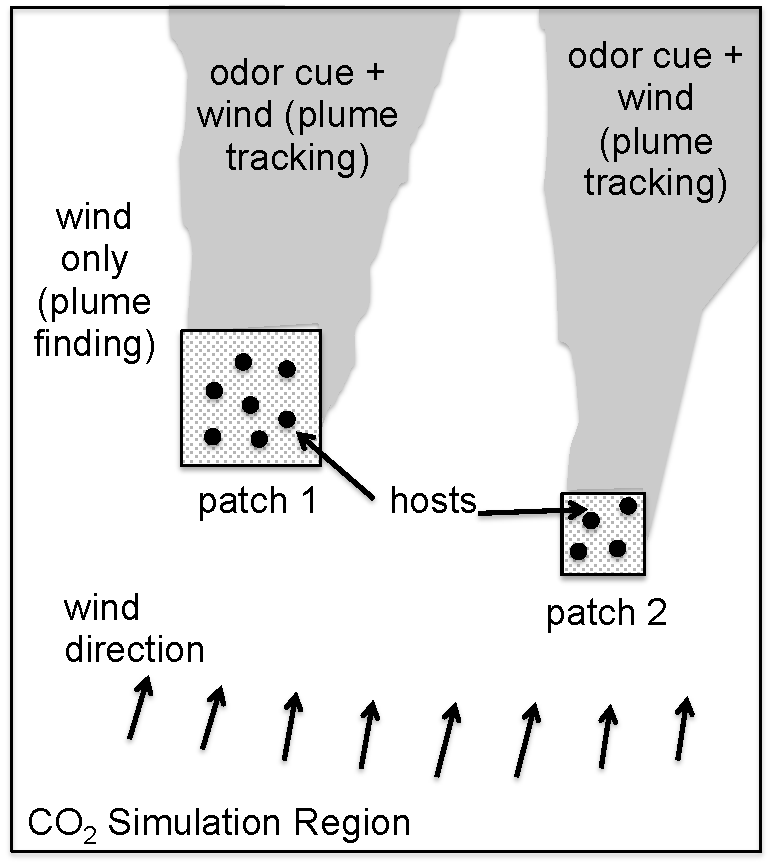
\includegraphics[width=3in]{revisedfigures/Figure1}
\caption{
{\bf Schematic of the type of host distributions considered in the model.}  The large rectangle is the 
CO$_2$ simulation region which is where the odor plume is computed.  At the edges of the simulation 
region, the CO$_2$ concentration is assumed to simply be carried out by the wind.  
The patches represent smaller subregions where the hosts are located.  We consider the spatial distribution 
of hosts within each patch to be uniform and there can be any number of patches. In the
simulations presented, the hosts are assumed to be stationary, although this is not a limitation of the model.
The mosquitoes are initially placed in a subregion inside the CO$_2$ simulation region but are allowed to 
leave it (and possibly reenter it) during the simulation. The wind, when included, exists everywhere where 
the mosquitoes move, even outside the CO$_2$ simulation region.}
\label{fig:setup}
\end{figure}
\end{center}


\begin{figure}[!htp]
% 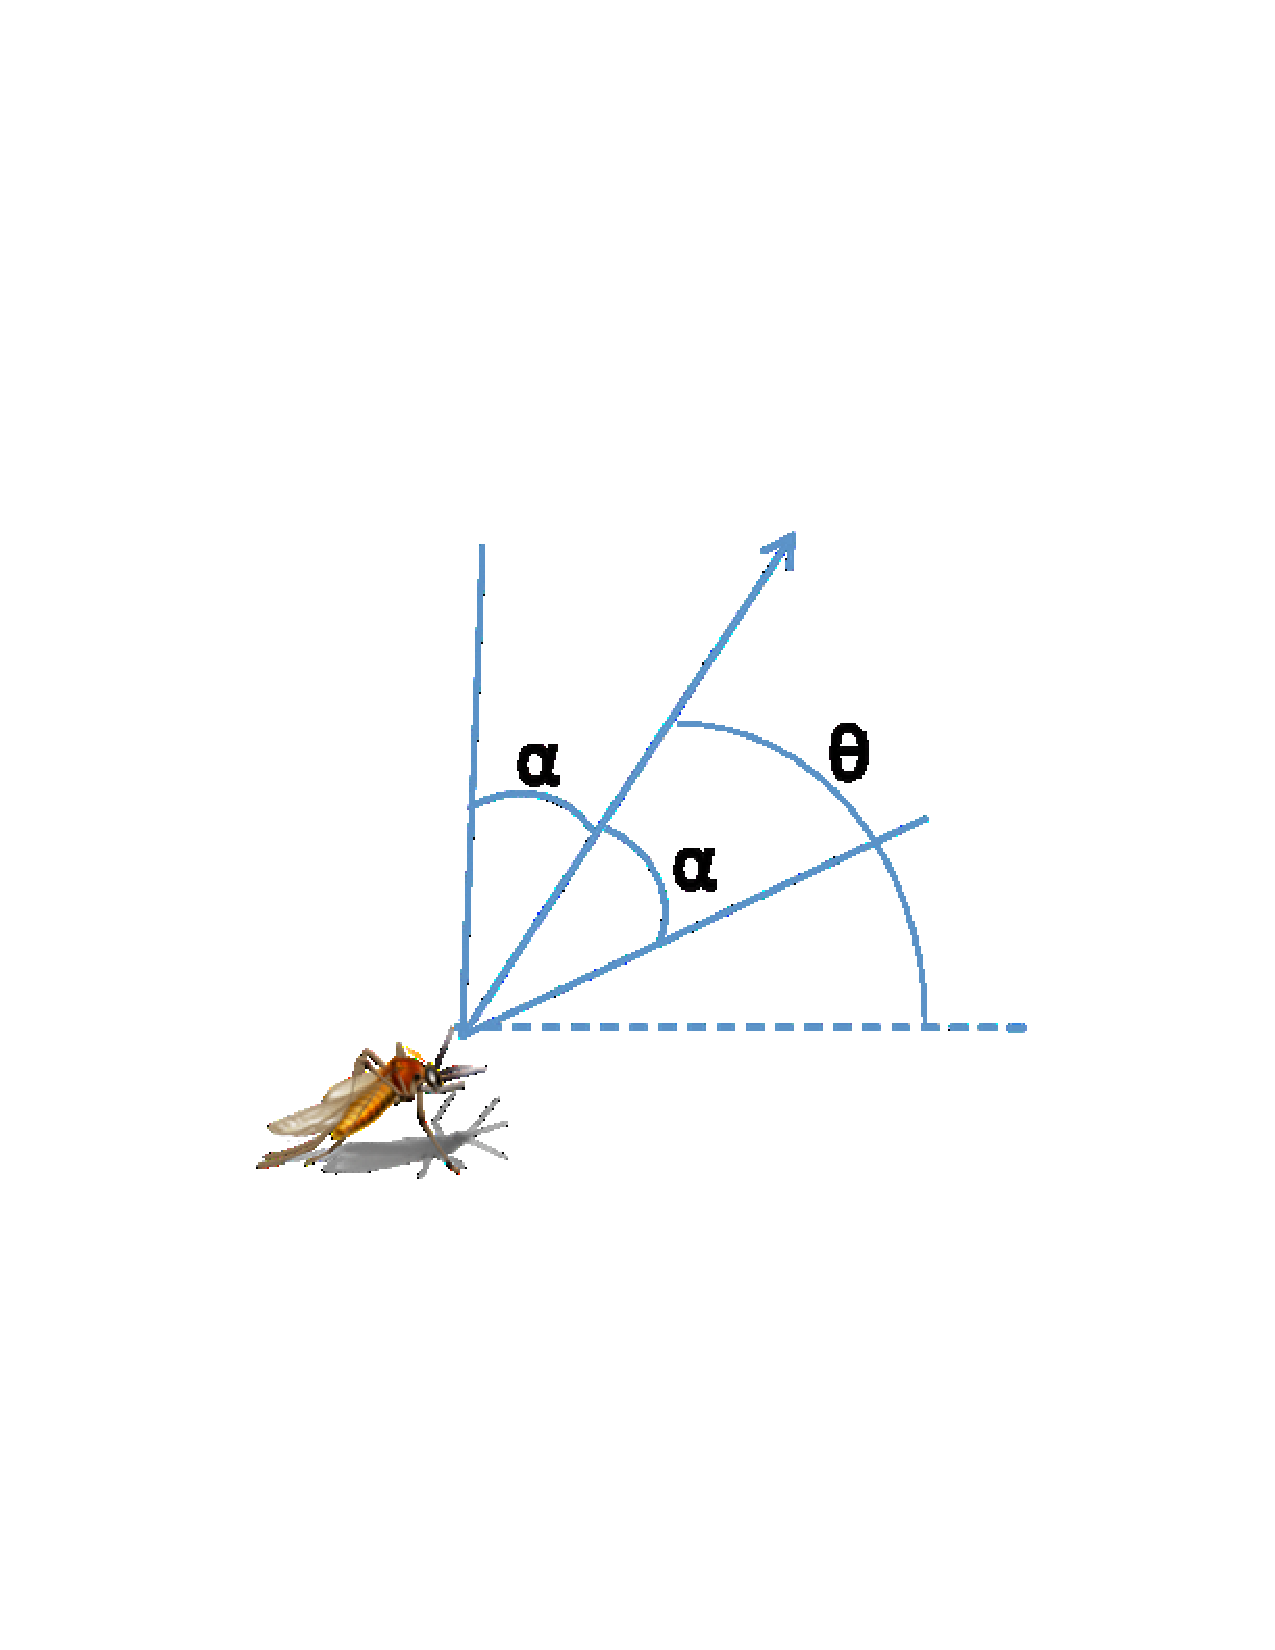
\includegraphics[width=2in]{revisedfigures/Figure2A} 	
% 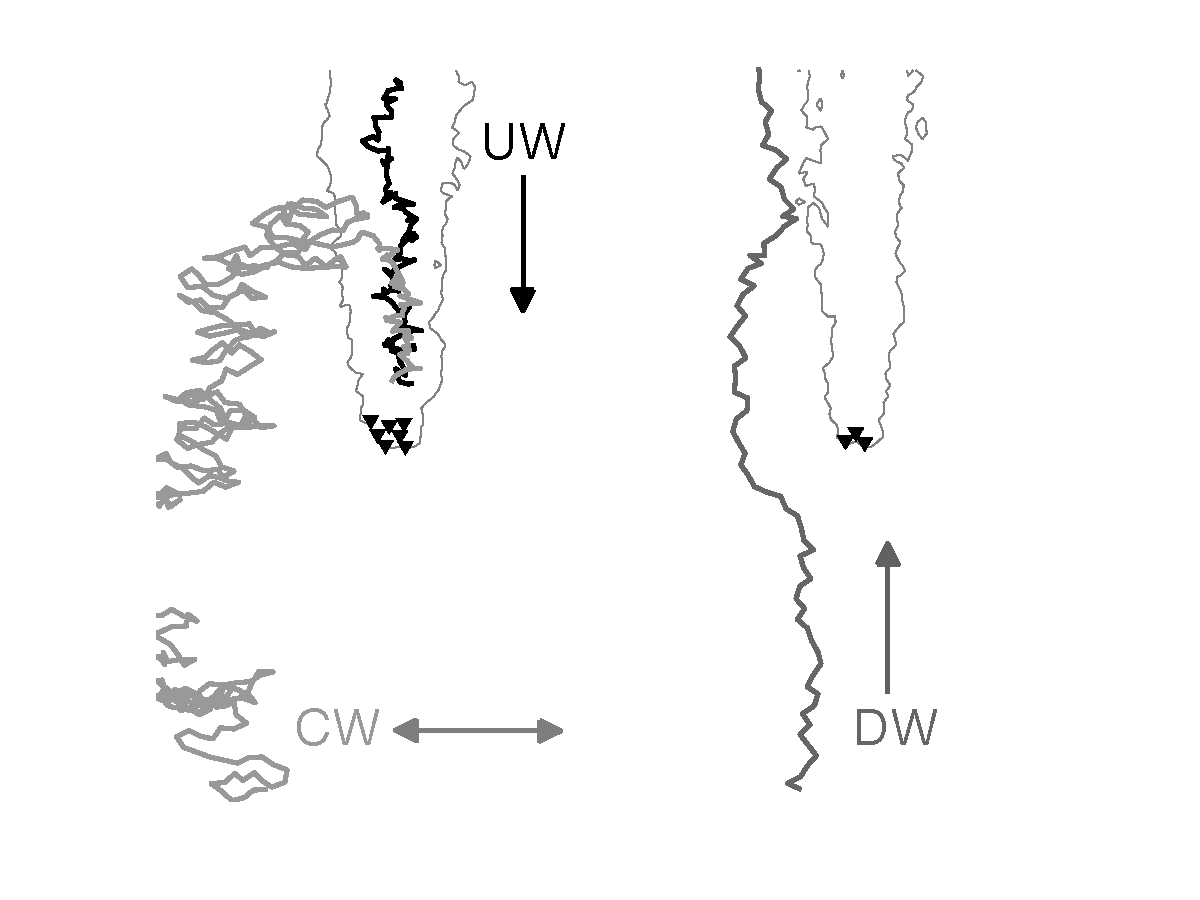
\includegraphics[width=4in]{revisedfigures/Figure2B}
\caption{
{\bf Mosquito flight direction choice and examples of mosquito trajectories. } A. Schematic of the mosquito direction choice in the host--seeking model. At each discrete flight segment, the angle $\theta$ represents the target direction of the mosquito -- the best possible direction it could choose given its information. However, the mosquito is only able to sense or to follow the target direction within a precision of $\alpha$.  B. Example mosquito trajectories for upwind (UW), downwind (DW), and crosswind (CW) plume finding behaviors. The stationary hosts are distributed into two groups with seven birds in the large group and three in the small. The contour of the odor plume marks the CO$_2$ sensing threshold of the mosquito at a single time. In reality, the shape of the plume changes over the course of the mosquito flight. The upwind mosquito begins within the plume of the large group and moves directly toward a host. The crosswind mosquito begins downwind of the large group, momentarily exits the domain but returns, finds the plume, and switches to an upwind strategy to track the plume. The downwind mosquito does not successfully encounter the small group's plume and exits the domain permanently.
}

\label{MosquitoGradient}
\end{figure}

\begin{figure}[!htp]
% 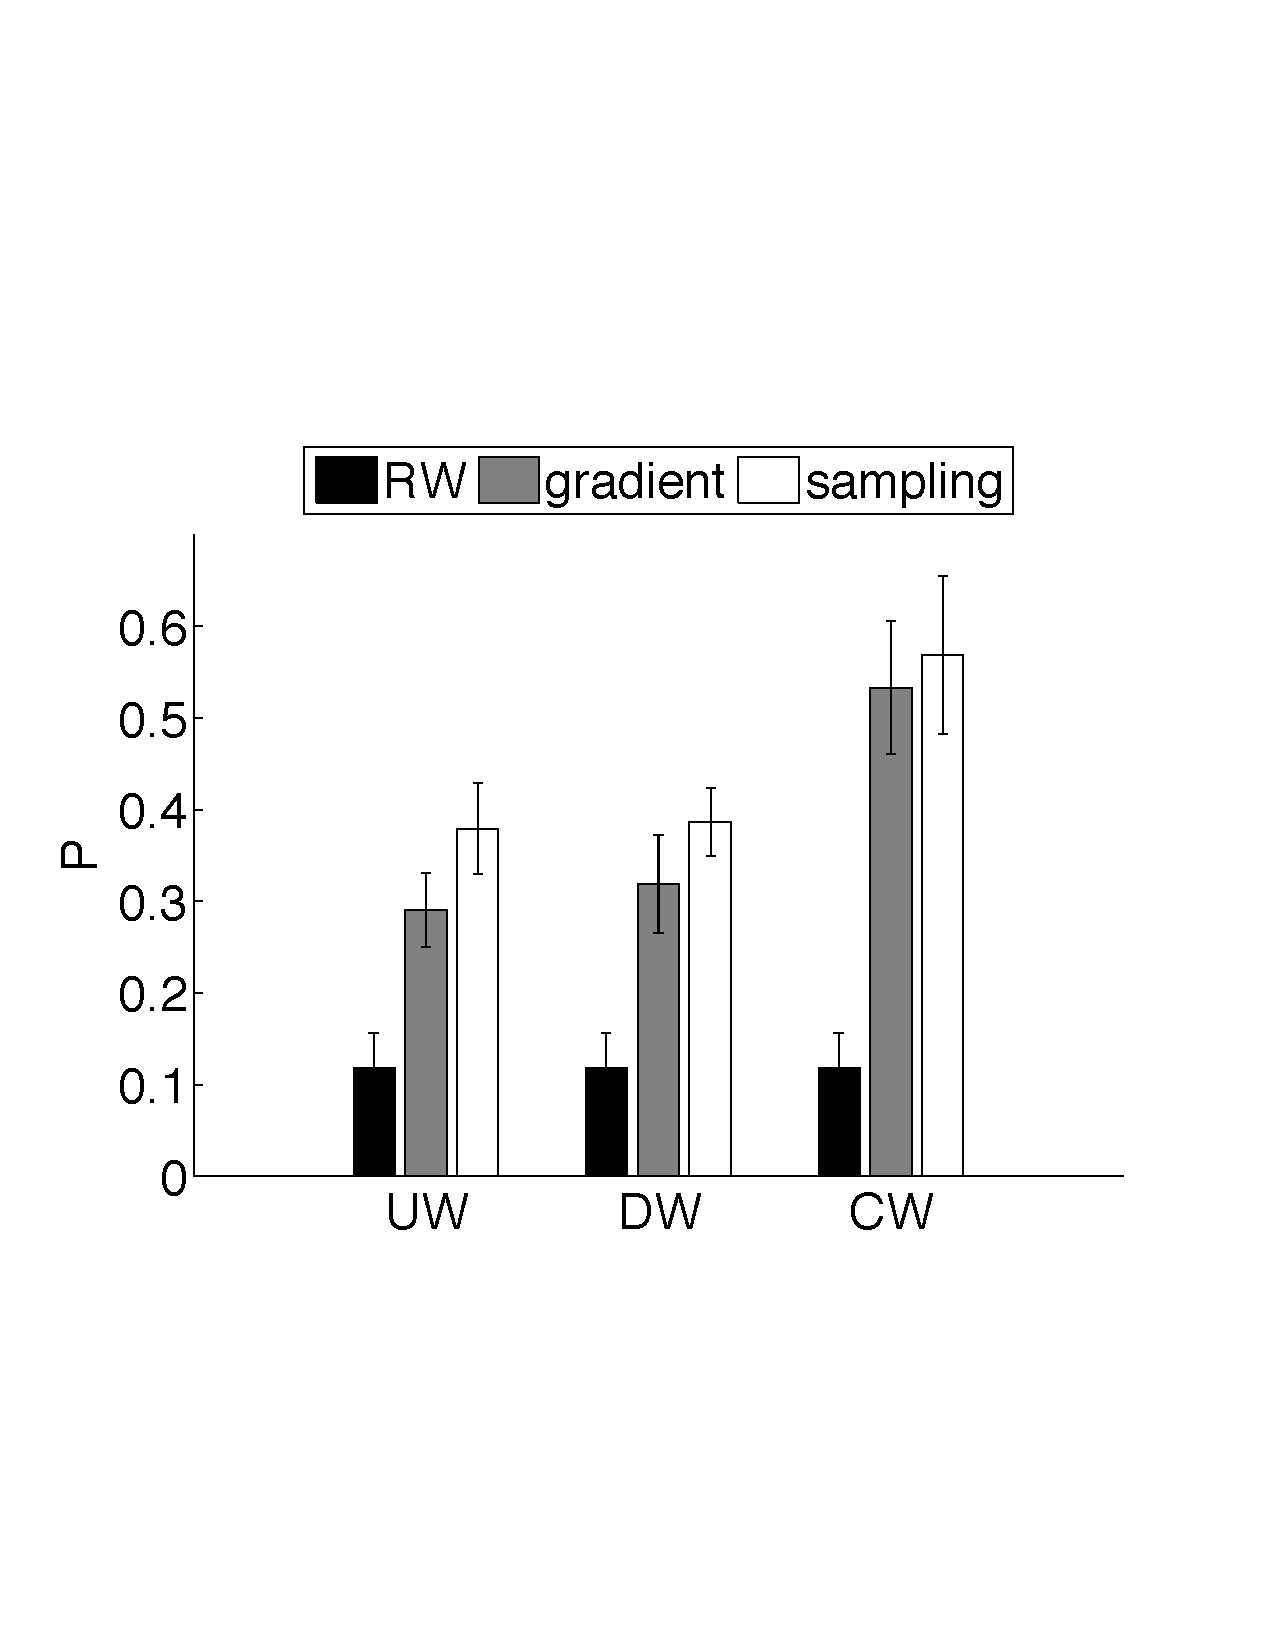
\includegraphics[width=4.5in]{revisedfigures/Figure3}
\caption{
{\bf The proportion of mosquitoes finding a host within 1500 navigation decisions.} The black bars are the results for a random walk (RW) without wind and CO$_2$, the gray for the gradient method of concentration sensing, and the white for the sampling method of concentration sensing. UW = upwind plume finding behavior, DW = downwind plume finding behavior, and CW = crosswind plume finding behavior. The thin error bars are $\pm$2 standard deviations. If the simulation is allowed to progress beyond 1500 decisions, then no appreciable changes occur in the results for the host--seeking methods, but the random walk continues to accrue contacts. }
\label{fig:rulecomp}
\end{figure}


\begin{figure}[!htp]
% 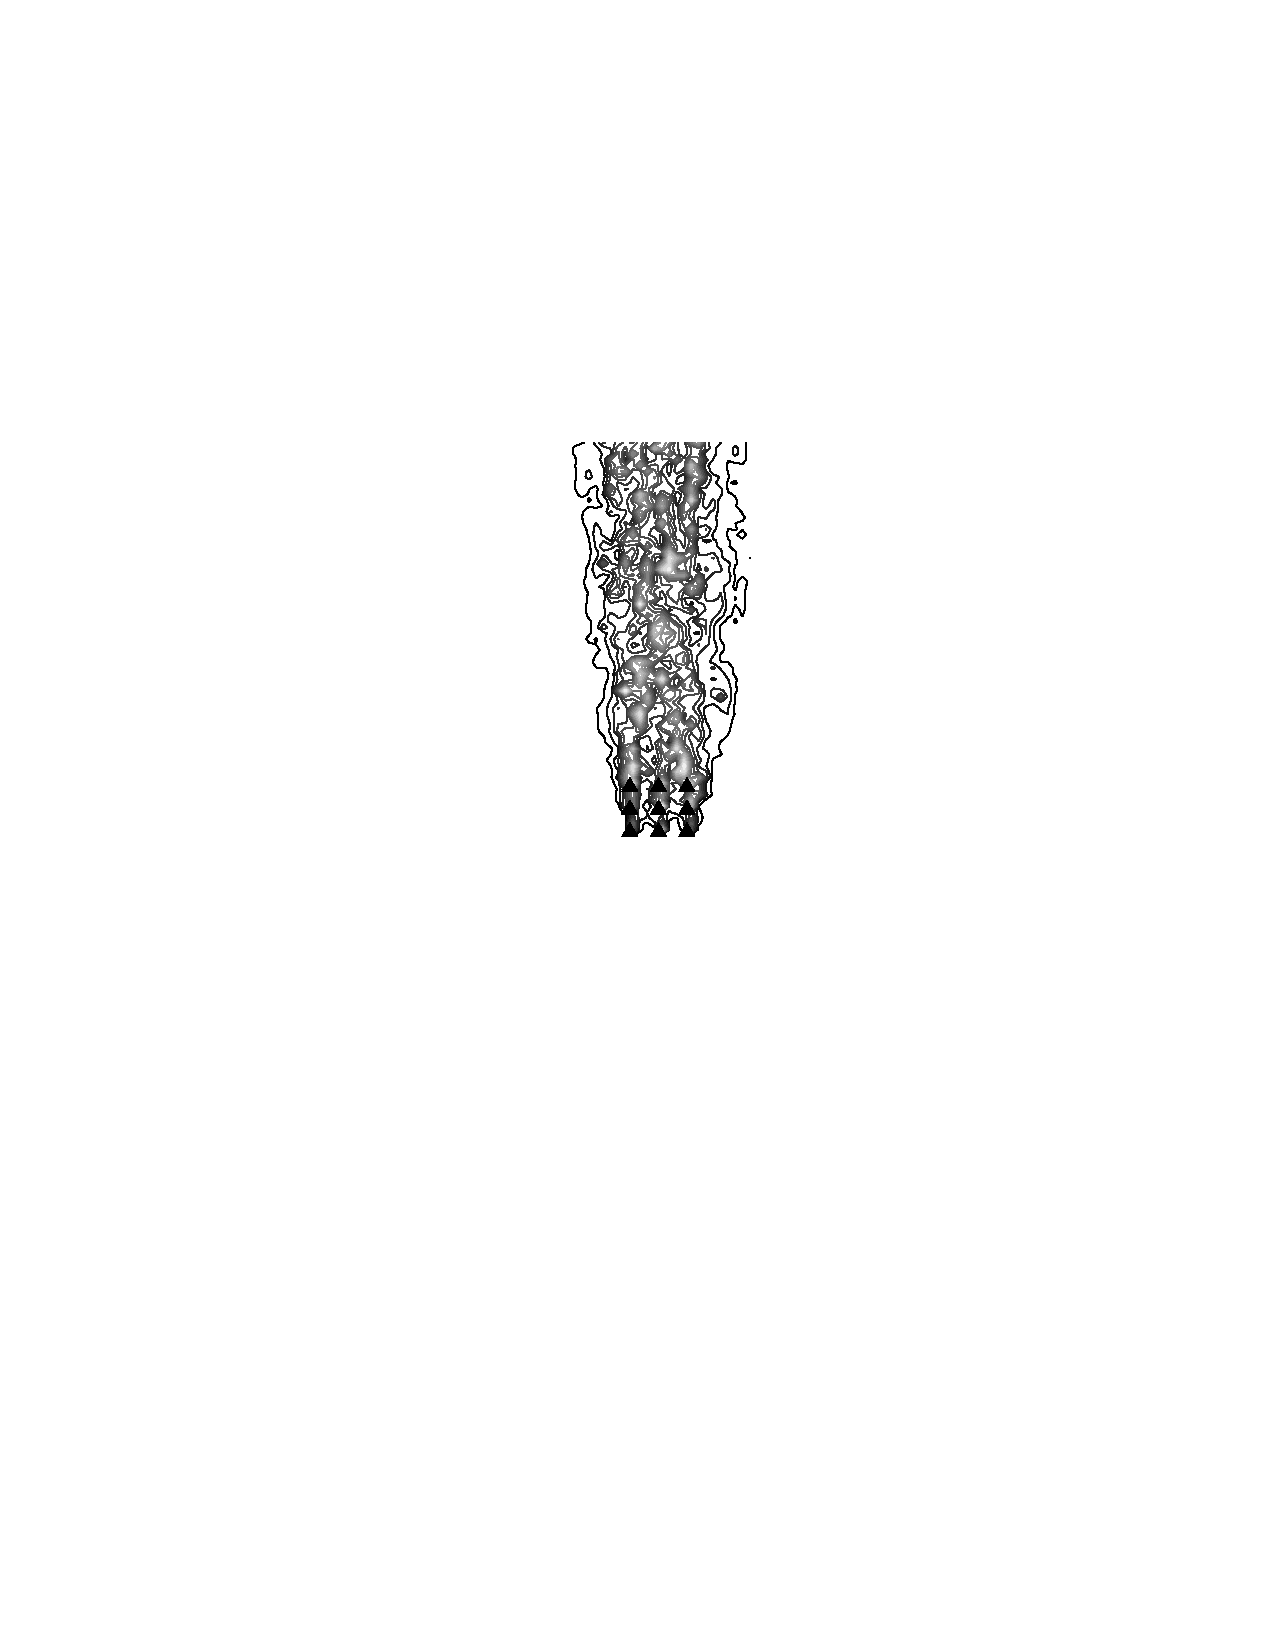
\includegraphics[width=3in]{revisedfigures/Figure4A}
% 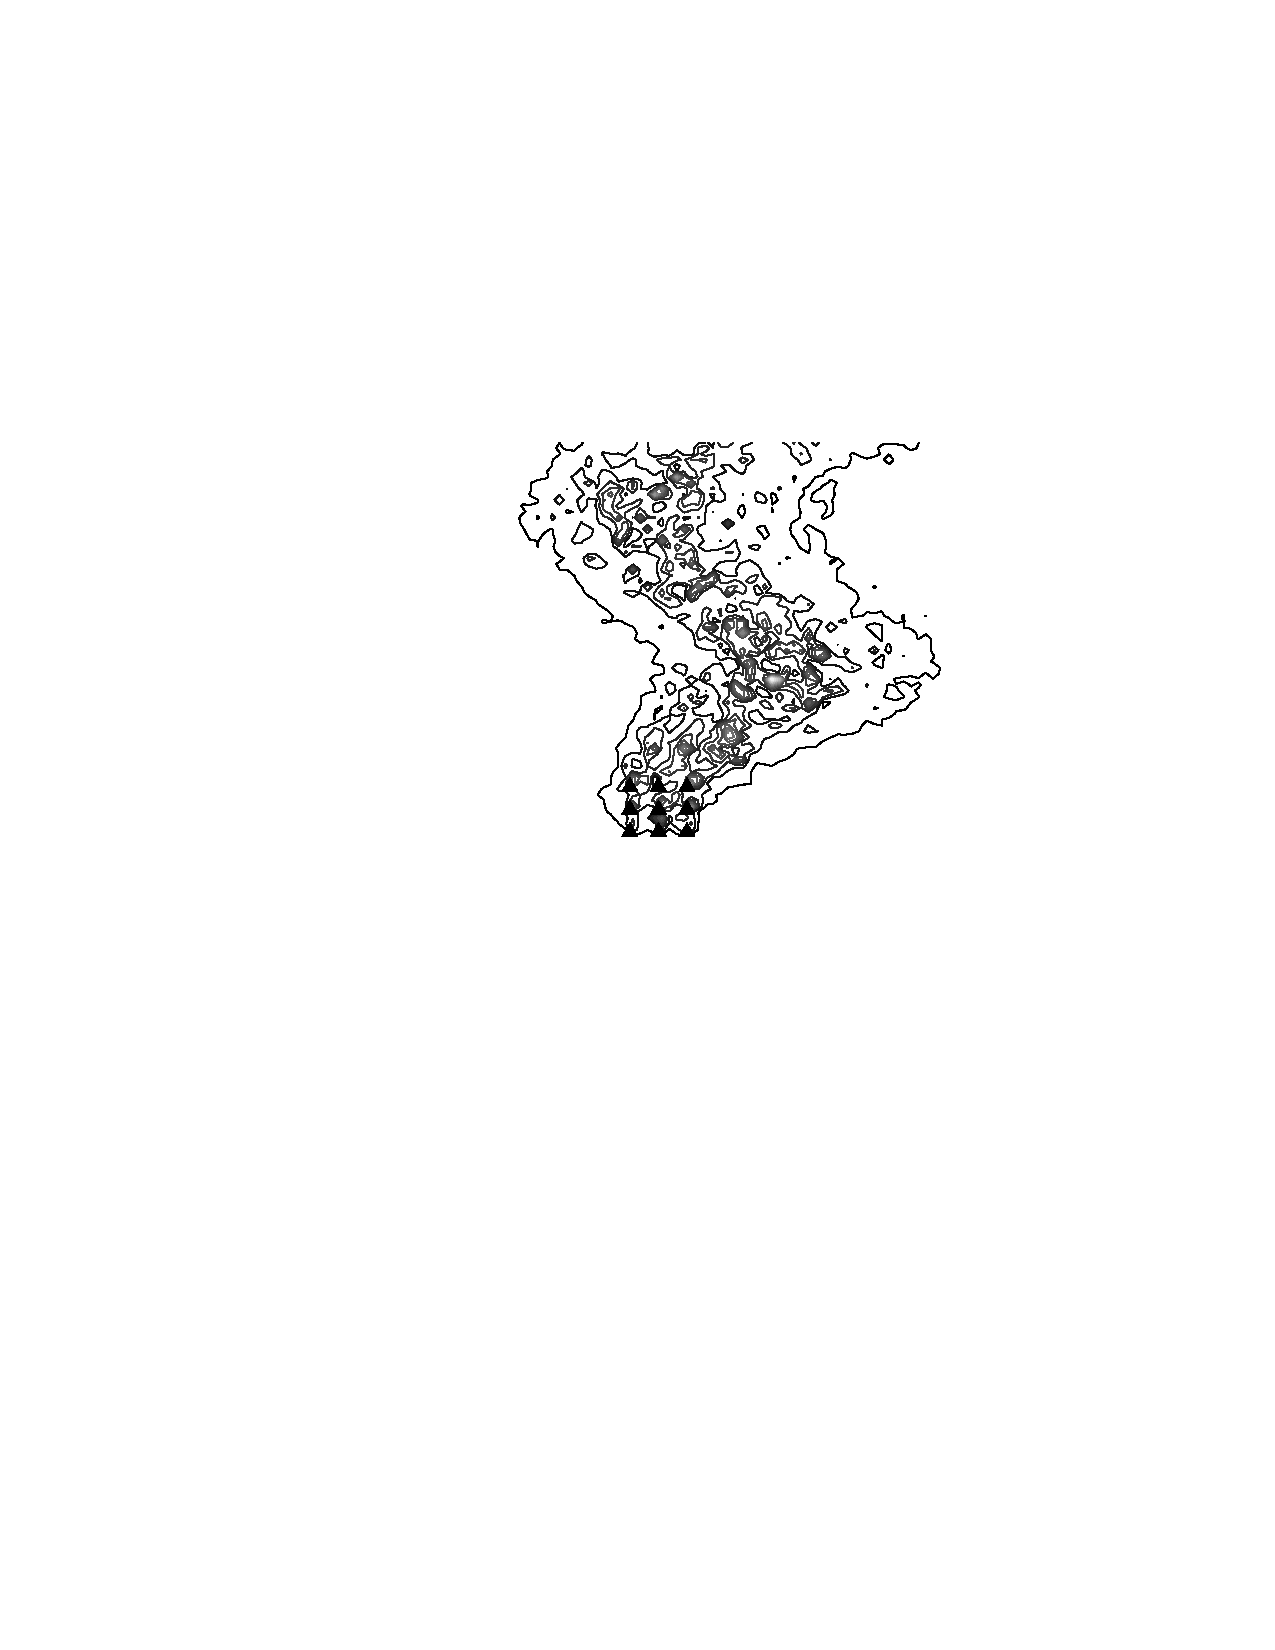
\includegraphics[width=3in]{revisedfigures/Figure4B}
\caption{
{\bf Examples of straight and meandering plumes with a superposed random velocity field.}  The triangles denote host position. The contours show concentration level, with darker bars indicating lower concentration. The lowest contour is $C_0$ and is the same in both plots. The other contours are not the same in both plots because the maximum concentration is roughly three times higher in the meandering plume.}
			\label{fig:Meander}
\end{figure}

\begin{figure}[!htp]
% 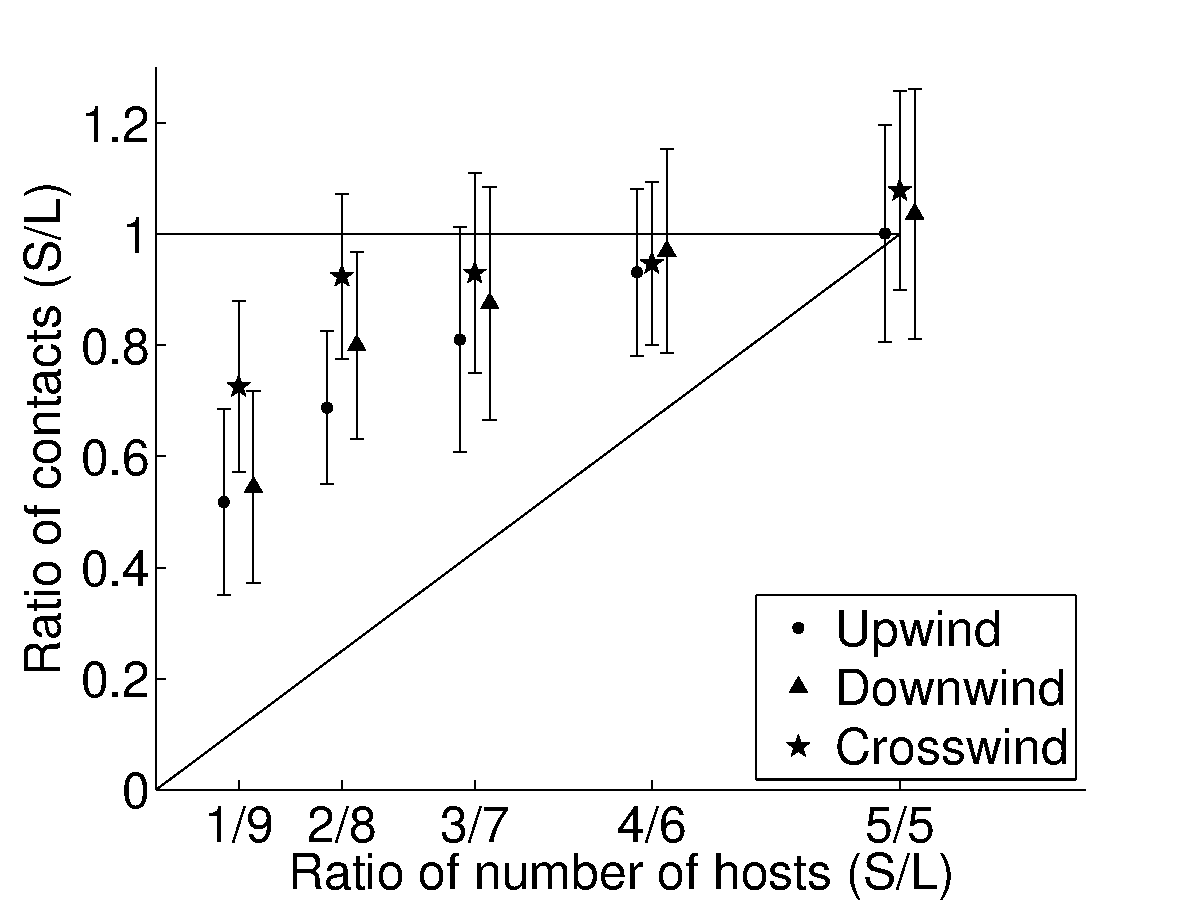
\includegraphics[width=4in]{revisedfigures/Figure5}
\caption{
{\bf Ratio of contacts between a small and a large host group.} Mean $\pm$ standard deviation of (\# contacts in the small group)/(\# contacts in the large group) plotted vs (\# hosts in the small group)/(\# hosts in the large group). The line $y=x$ shows an equal per capita contact rate between groups. Equality is not achieved until the group sizes are equal (or nearly so).  The data corresponding to a given ratio of hosts have been separated
	slightly in the figure for visual purposes only.}
	\label{fig:2groupsres}
\end{figure}

\begin{figure}[!htp]
% 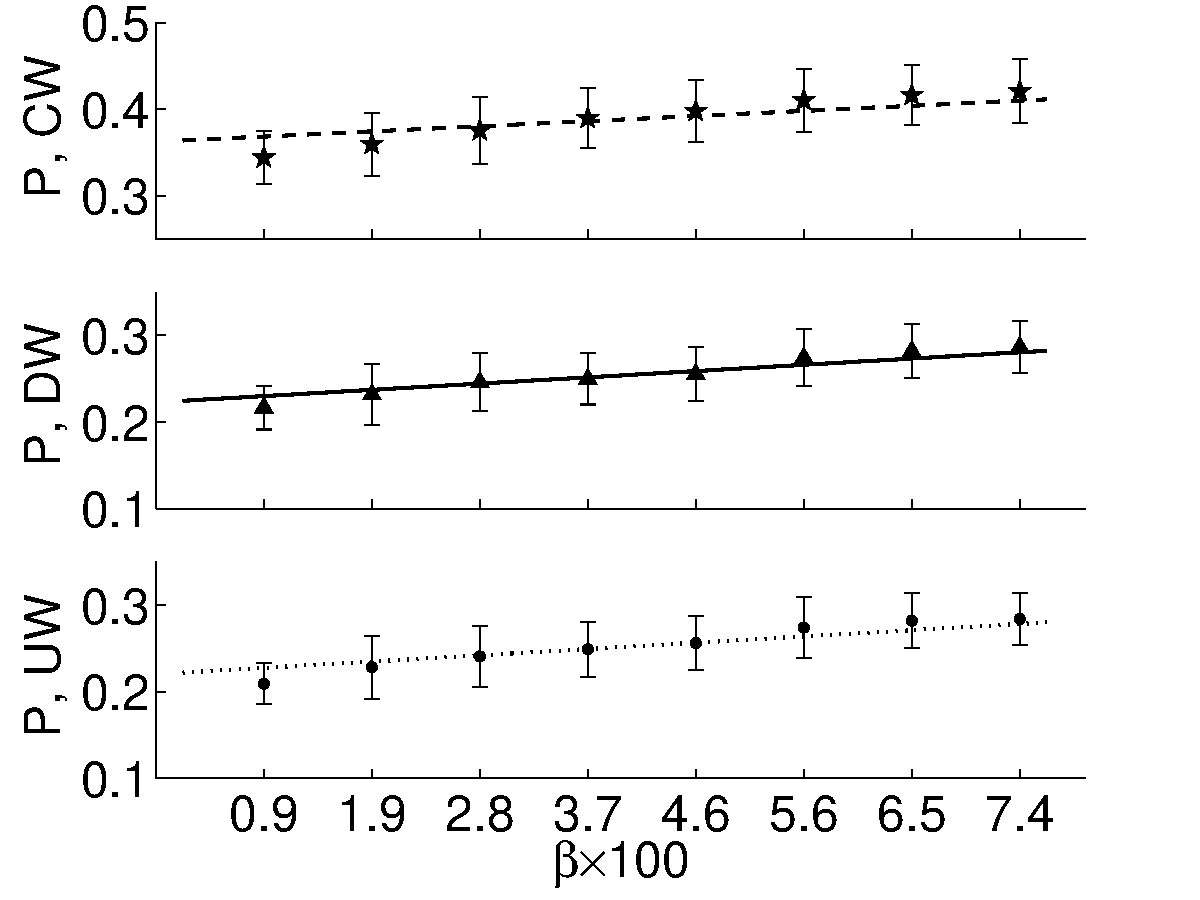
\includegraphics[width=3in]{revisedfigures/Figure6}
\caption{
{\bf The proportion of mosquitoes finding a host as a function of host density.} The simulation results are given by the solid markers with $\pm$ one standard deviation (UW = upwind, DW = downwind, CW = crosswind). The lines are linear fits to the data using the formula $P = P_0 + \beta(1-P_0)$, where $\beta$ is the area of the host patch divided by the area of the simulation region (the proportion of the domain covered by hosts). As $\beta$ increases, the hosts spread out (i.e., decrease in density) and the number of mosquitoes locating a host increases. The $x$-axis is $\beta$ multiplied by 100 for ease of viewing, since $\beta$ is quite small. }
	\label{fig:Density}
\end{figure}

\newpage
\section*{Tables}
		
\begin{table}[!htp]
\caption{
{\bf Parameter choices.} *Starred values were locally varied. The second column has the nondimensional values used in the simulations. The third contains the associated dimensional values using the characteristic quantities given in the Methods section.}
	\begin{center}
		\begin{tabular}{|c|c|c|l|}
			\hline
			\multicolumn{4}{|c|}{Mosquito speed in the presence of CO$_2$, $b=C/C_{sat}$} \\
			\hline 
			symbol & dimensionless value & dimensional value & description \\
			\hline
			$S_{min}$ & 0.4* & 0.4 m/s & minimum mosquito flight speed\\
			$S_{max}$ & 1.5* & 1.5 m/s & maximum mosquito flight speed\\
			$C_0$ & 0.01* & 40 ppm & CO$_2$ sensing threshold (no ambient CO$_2$)\\
			$C_{sat}$ & 1 & 4000 ppm & CO$_2$ sensing saturation (no ambient CO$_2$)\\
			\hline \hline
			\multicolumn{4}{|c|}{Mosquito CO$_2$ direction, $b=|C_{n}-C_{n-1}|/\Delta C_{sat}$} \\
			\hline 
			symbol & dimensionless value & dimensional value & description \\
			\hline
			$\alpha_{min}$ & $\pi/36$* & $\pi/36$ & minimum interval width for $\Delta C$\\
			$\alpha_{max}$ & $\pi$  & $\pi$ & maximum interval width for $\Delta C$\\
			$\Delta C_0$ & $5\times10^{-5}$  & 0.2 ppm & $\Delta C$ sensing threshold\\
			$\Delta C_{sat}$ & $0.02$  & 80 ppm & $\Delta C$ sensing saturation\\
			\hline \hline
			\multicolumn{4}{|c|}{Mosquito wind direction, $b=|\vec{V}|/V_{sat}$} \\
			\hline 
			symbol & dimensionless value & dimensional value & description \\
			 \hline
			$\alpha_{min}$ & $\pi/6$* & $\pi/6$ & minimum interval width for wind direction \\
			$\alpha_{max}$ & $\pi/2$ & $\pi/2$ & maximum interval width for wind direction \\
			$V_0$ & 0 & 0 m/s & wind sensing threshold\\
			$V_{sat}$ & 0.5 & 0.5 m/s & wind sensing saturation\\
			\hline \hline
			\multicolumn{4}{|c|}{Wind parameters} \\
			\hline 
			symbol & dimensionless value & dimensional value & description \\
			\hline
			$U_2$ & 0.2 & 0.2 m/s & speed of large--scale flow\\
			$\vec{U}_r$ & [X(t), Y(t)]0.15* & [X(t), Y(t)]0.15 m/s & superposed random flow field \\[5pt]
			\multirow{2}{*}{$X(t),Y(t)$} & \multirow{2}{*}{mean 0, std dev 0.5} & \multirow{2}{*}{mean 0, std dev 0.5}&
			normally distributed random variables  \\
			& & & changed every 20 $\Delta T$ (2 s)\\
			\hline \hline
			\multicolumn{4}{|c|}{Miscellaneous constants} \\
			\hline 
			symbol & dimensionless value & dimensional value & description \\
			\hline
			$D$ & 1.6$\times 10^{-4}$* & 1.6$\times 10^{-5}$ m$^2$/s& diffusion coefficient\\
			$J_0$ & 0.042* & 1680 ppm/s & source coefficient\\
			$r_c$ & 5* & 0.5 m & critical radius for mosquito-host contact  \\
			$L$ & 100 & 10 m & length of a side of the square domain \\
			$T_f$ & up to 5000 & up to 500 s & length of the simulation \\
			$N_v$ & 200 & 200 & number of mosquitoes per simulation \\
			$T_{cwd}$ & $\Delta T$[5, 9]* & [0.5, 0.9] s & 
			duration of crosswind flight  \\
			\hline
		\end{tabular}
	\end{center}\label{tab:finalparams}
\end{table}


\begin{table}[!htp]
\caption{
{\bf Most sensitive local variation.} This table lists the highest sensitivity indices that we found over all plume finding behaviors, input parameters, and output variables for the test problem described in the text. The second column has the name of the output variable being measured and its value at the unvaried parameter set given in  Table~\ref{tab:finalparams}. Input parameters that caused the highest sensitivity indices are in column three. $P$ is proportion of mosquitoes that found a host and $T_{avg}$ is average number of navigation decisions a mosquito makes before finding a host. The fourth and fifth columns are the sensitivity index and its error (see the text for details of calculation). If the absolute value of $SI$ is much less than 1, then the measured output \textit{is not sensitive} to small variations in the input parameter. All combinations of plume finding behavior, input parameter, and output variable not given in this table have $|SI| < 0.3$. }
	\begin{center}
		\begin{tabular}{|c|c|c|c|c|}
			\hline
			plume finding behavior & output (baseline value) & input & $SI$ & $SI$ Error \\
			\hline
			\multirow{2}{*}{upwind} & \multirow{2}{*}{$T_{avg}$ (116)} & $S_{max}$  &  -1.8139 & 0.3155 \\
										& 						  & 	$J_0$&    0.3035 & 0.1661 \\
			\hline
			\multirow{5}{*}{downwind} & \multirow{3}{*}{$T_{avg}$ (46)} & $S_{max}$  & -0.6432 & 0.6093\\
										&								& $r_c$		&  -1.0265 & 0.8221\\						
										& 						  & 	$C_0$		&   -0.6312 & 0.6741\\
										\cline{2-5}
										 & \multirow{2}{*}{$P$ (0.20)}	& \multirow{2}{*}{$r_c$}  & \multirow{2}{*}{0.3156} & \multirow{2}{*}{0.0374}\\
										&&&&\\
			\hline
				\multirow{2}{*}{crosswind} & \multirow{2}{*}{$P$ (0.36)}	& \multirow{2}{*}{$S_{max}$} & \multirow{2}{*}{0.7292}  & \multirow{2}{*}{0.2666}\\
			&&&&\\
			\hline
		\end{tabular}
	\end{center}\label{tab:sensitivity}
\end{table}


\begin{table}[!htp]
\caption{{\bf A comparison of plume finding behaviors in straight and meandering plumes.} The third and fourth columns, $P$ and std dev, are the average and standard deviation of the proportion of mosquitoes finding a host taken over 15 simulations of the same plumes with stochastic mosquito behavior. Each simulation is sufficiently long to ensure that all the mosquitoes either find a host or leave the domain. The ``$T_{avg}$'' column is the average number of navigation decisions a mosquito makes before finding a host (average taken over all simulations). The associated standard deviation taken over the \textit{means} of the simulations. The final column recalculates $P$ assuming that the simulation halts after 350 mosquito decisions.}
	\begin{center}
		\begin{tabular}{|c|c|c|c|c|c|c|}
			\hline
			plume finding behavior & plume type &$ \quad P \quad $& std dev & $T_{avg}$ & std dev & $\quad P_{350} \quad$\\
			\hline
			\multirow{2}{*}{upwind} & straight &22\% & 1.7\% & 116 & 5 & 22\%\\
										&  meander & 38\% & 2.5\% & 159 & 4 & 38\%\\
										\hline
			\multirow{2}{*}{downwind} & straight &20\% & 1.8\% & 46 & 9 & 20\%\\
										&  meander & 39\% & 1.9\% & 97 & 6 & 38\%\\
										\hline
			\multirow{2}{*}{crosswind} & straight &35\% & 3.5\% & 285 & 14 & 27\%\\
										&  meander & 57\% & 4.2\% & 569 & 20 & 14\%\\
			\hline
		\end{tabular}
		\label{tab:meander}
	\end{center}
\end{table}






\end{document}

